\documentclass[11pt, titlepage]{article}
\usepackage{psdiproject_report}
\usepackage{mhchem}
\usepackage{siunitx}
\renewcommand{\familydefault}{\sfdefault}
\usepackage{tabularx}
\usepackage{amsmath}
\hypersetup{citecolor=blue, urlcolor=cyan}

%%%%%%%%%%%%%%
%Instructions%
%%%%%%%%%%%%%%
%Edit the section below replacing the capitalised text with the information for the specific report
%Complete the sections of the report as necessary
%%%%%%%%%%%%%%

%%%%%% EDIT THIS SECTION %%%%%%
%replace the capitalised text with the relevant information - don't remove the \xspace
\newcommand{\projectname}{Modelling Phase Transitions: Characterising Henry's Law\xspace} %INSERT PROJECT NAME HERE
\newcommand{\projectdates}{24th June - 30th August 2024\xspace} %AMEND PROJECT DATES AS NECESSARY
\newcommand{\studentlist}{Joshua Cheung\xspace}  %INSERT STUDENT NAME HERE
\newcommand{\reportdate}{30/08/2024\xspace} %INSERT PUBLISHED DATE HERE dd/mm/yyyy
\newcommand{\reporttitle}{PSDI-Intern-Series-2024:Report\_1\xspace} %report number do not change
\newcommand{\doi}{DOI HERE} %INSERT DOI HERE - PSDI Team will provide this

%%%%%
\begin{document}
\renewcommand{\arraystretch}{1.5}

%%%%%%TITLE PAGE%%%%%%
\PSDITitlePage{}
%%%%%PUBLISHING INFO%%%%%
\publishinginfo{}
%%%%%Contents%%%%%
\PSDIContents{}

\setcounter{page}{1}
\section{Project Details}

\begin{table}[H]
\centering
\begin{tabular}{|p{1.5in}|p{4.5in}|}
\hline %row no:1
\textbf{Project Name} & {\projectname} \\ %if necessary change in details section at beginning of document
\hline %row no:2
\textbf{Project Dates} & {\projectdates} \\ %if necessary change in details section at beginning of document
\hline %row no:3
\textbf{Website} & 
\href{xxx}{\url{https://github.com/joooshc/PSDI_HLC}} \\ %insert project website if applicable
\hline
\end{tabular}
 \end{table}

\subsection{Project Student}
\begin{table}[H]
	\centering
	\begin{tabular}{|p{2in}|p{4in}|}
		\hline
		%row no:1
		\textbf{Name and Title} & Joshua Cheung \\ %insert name and title here 
		\hline
		%row no:2
		\textbf{University Department Name} & 
		School of Chemistry and Chemical Engineering \\ % Employer name/University Department Name here
		\hline
		%row no:3
		\textbf{Work Email} & 
		jc10g22@soton.ac.uk \\ %work email here
		\hline	
	\end{tabular}
\end{table}

\subsection{Project Supervisors}
%%%%%%%%% 
%(Please add/delete boxes to meet the number of co-investigators you have. NB: If any have been added please mark them as new and include the date they started on the project)
%%%%%%%%%
\begin{table}[H]
	\centering
	\begin{tabular}{|p{2in}|p{4in}|}
		\hline
		%row no:1
		\textbf{Name and Title} & Professor Jeremy Frey \\ %insert name and title here 
		\hline
		%row no:2
		\textbf{University Department Name} & 
		School of Chemistry and Chemical Engineering \\ % Employer name/University Department Name here
		\hline
		%row no:3
		\textbf{Work Email} & J.G.Frey@soton.ac.uk \\ %work email here
		\hline
	\end{tabular}
\end{table}

\begin{table}[H]
	\centering
	\begin{tabular}{|p{2in}|p{4in}|}
		\hline
		%row no:1
		\textbf{Name and Title} & Dr. Joanna Grundy \\ %insert name and title here 
		\hline
		%row no:2
		\textbf{University Department Name} & 
		School of Electronics and Computer Science \\ % Employer name/University Department Name here
		\hline
		%row no:3
		\textbf{Work Email} & J.Grundy@soton.ac.uk \\ %work email here
		\hline
	\end{tabular}
\end{table}

\subsection{Project Description}
\label{subsec:ProjectDescription}
%\textit{Guidance (Delete upon completion): Please provide a short summary of the project you undertook in your internship. Some of this content can be taken from the initial internship descriptions.}
Aqueous solubility is a highly important property in a range of scientific areas, ranging from mass production of chemicals in industry, to drug design\cite{DrugSolubility} and flow synthesis\cite{FlowChemistry}. Measured as $\log (\text{mol dm}^{-3})$ and denoted as $\log S$, it describes the amount of a solute that is dissolved in a solvent. Related to this is Henry's law constant ($k_H$), in units of $\frac{\text{mol}}{\text{atm}}$, which describes the proportion of a gas that is dissolved in a liquid\cite{Sander}.

Despite its importance, existing computational methods for predicting Henry's law constant are largely restricted to semi-empirical methods, and there is a significant lack of experimentation with machine learning. During the past 15 years, interest has started to arise in the use of machine learning to predict solubility\cite{Llompart2024}, and this project hopes to expand this to the prediction of Henry's law constant.

In this project, data was curated from several sources of data to create a master dataset consisting of $\log S$, $k_H$, and a corresponding temperature, as well as chemical identifiers. A diverse assortment of data preparation methods were assessed, including normalization, feature selection based on variance, and SelectKBest. Various machine learning algorithms, such as LightGBM and K-Nearest Neighbours (KNN), were trialled for predicting {$\log S$} and {$k_H$} values.

The overall objective of this project was to experiment with machine learning for the prediction of {$\log S$} and {$k_H$}, and explore the links between them.

\section{Lay Summary}
\label{sec:LaySummary}
%\textit{Guidance (Delete upon completion): Please provide a short publicity summary of the work you did to complete this project. This should be understandable by a general audience}

The main focus of this project was to use machine learning models to predict values for solubility ($\log S$) and Henry's law constant ($k_H$), exploring the links between the two properties. These properties are highly important in a variety of fields, such as drug design\cite{DrugSolubility}, modelling environmental systems\cite{EnvironmentHL}, understanding decompression sickness\cite{GasLaws}, as well as flow chemistry\cite{FlowChemistry}.

Data was curated and processed to form a dataset with over 21 000 datapoints, which was used to train and test an assortment of machine learning models. Overall, the most accurate model for both properties was the LightGBM Gradient Boosting Regressor\cite{LGBMRegressor}, which combines the results from sub-models to learn progressively and improve results. 

Many data-related challenges were faced, ranging from data scarcity, to subpar data quality (e.g. missing identifiers, missing temperatures, extreme values). The vast majority of the datapoints were at standard temperature (25$^\circ$ C), and all were assumed to be at standard pressure. It is highly likely that the models will not perform well at other temperatures. Regardless, two machine learning models were successfully used to predict solubility and Henry's law constant for a wide range of compounds in aqueous solution.

\section{Introduction}
\label{sec:Introduction}
%\textit{Guidance (Delete upon completion): Please provide a short introduction to this report. This should include some background information based on literature and other relevant material,  motivation behind the project,  the project aims and objectives,  the  project scope (what you have and haven't achieved) and a brief summary of what the rest of the report covers}

Henry's law, discovered in 1803 by William Henry\cite{Henry1803}, suggests that the solubility of a gas in a given solvent is `proportional to its partial pressure in the gas phase'\cite{Sander}. This statement is valid in the limits of infinite dilution of the solute when the gas is considered ideal\cite{HL_IUPAC_Recs}. For an ideal-dilute solution (a solution where the solvent follows Raoult's law and the solute follows Henry's law), Henry's constant can be calculated using the following equation, where $x_A$ is the mole fraction of the solute, $k_H$ is Henry's law constant with dimensions of pressure, and $p_A$ is the pressure\cite{Atkins}.
\begin{equation}
	p_A = x_A k_H
	\label{eq:HenrysLaw}
\end{equation}
The name `constant', is a misnomer; it is not a true constant, and is dependent on temperature. In truth, Henry's law constant is actually a proportionality constant, as is seen in the format of the equation. As a general rule, it has a somewhat quadratic trend where it increases at low temperatures to a maximum, then decreases at high temperatures\cite{HLPitfalls}. 

\begin{figure}[H]
	\centering\small
	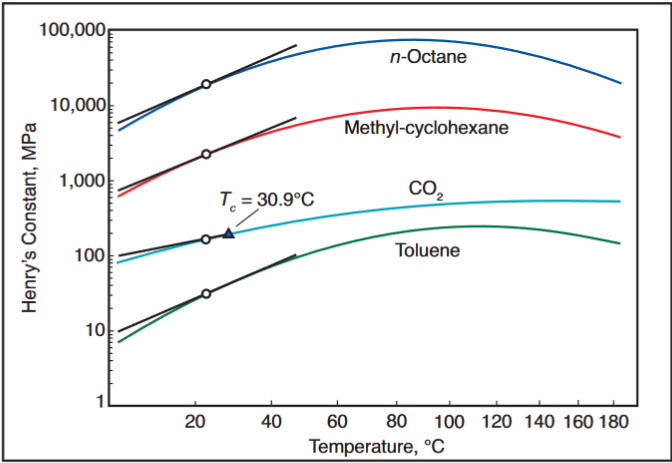
\includegraphics[width=0.5\linewidth]{figures/HenryTemp.png}
	\caption{The temperature dependence of some organic solutes in water. The x axis is linear when plotted as 1/T. Figure taken from \textit{Smith et al}\cite{HLPitfalls}.}
	\label{fig:HenryTemperatureDependence}
\end{figure}

Since Henry's law extrapolates to infinite dilution, it cannot be measured directly, increasing complexity.

Henry's law constant can also be defined in relation to the liquid and gas phase abundances, which is described as Henry solubility\cite{HL_IUPAC_Recs}. In this work, the terms `Henry solubility' and `Henry's law constant' are used interchangeably. The unit used was $\frac{\text{mol}}{\text{m}^3\text{ Pa}}$.
\begin{equation}
	K_{Hs} = \frac{Q_l}{Q_g}
	\label{eq:HenrySolubility}
\end{equation}

Solubility describes the composition of a saturated solution in terms of the quantity of a defined solute in a solvent\cite{IUPAC_SolubilityDefinition}. In 1887, François Marie Raoult published an article detailing a series of  experiments in which he measured the dependence of the vapour pressure of a solution on the quantity of a given solute in solution\cite{APS_Raoult, RaoultTranslation}. Rault's law states that `the ratio of the partial vapour pressure of each component to its vapour pressure when present as the pure liquid, is approximately equal to the mole fraction of A in the liquid mixture.'\cite{Atkins}
\begin{equation}
	p_A = x_A p^*_A
	\label{eq:RaoultsLaw}
\end{equation}

Henry's law constant can be approximated for a case where the solute is almost immiscible by combining Raoult's law and Henry's law\cite{HLPitfalls}:
\begin{equation}
	H = \frac{(1-x_w)p_A}{x_A}
	\label{eq:CombinedHenryRaoult}
\end{equation}
Here (equation \ref{eq:CombinedHenryRaoult}), $x_w$ is the mole fraction of water in the organic phase, $x_A$ is the mole fraction of the solute in the aqueous phase, and $p_A$ is the vapour pressure of the solute.

In cases where the solute is significantly more miscible, the derivation originates from equation \ref{eq:HenrysLaw}, but requires analysis of the phase equilibrium. This consists of fitting a liquid-activity model to the data and extrapolating to infinite dilution\cite{HLPitfalls}. 
\begin{equation}
	k_H = \gamma_A^{\infty} p_A
\end{equation}
More broadly speaking, both Henry's law constant (solubility) and solubility refer to the ability of a solute (gas or liquid) to dissolve in a given solvent.

Solubility, and Henry Solubility, are highly important chemical properties for a wide range of areas. Arguably, the most crucial of these areas is drug solubility. The solubility of a drug must be known to ensure that the correct amount of the drug is circulated throughout the body\cite{DrugSolubility}. As the human body is up to 75\% water by body weight\cite{WaterInBody}, it's essential that a drug must be able to dissolve in water to correctly be absorbed in the body to have a therapeutic effect.  Furthermore, there are many environmental issues relating to the solubility of pollutants, such as water soluble polymers in freshwater\cite{WaterPollution}, and the solvation of excess $\ce{CO2}$ in the oceans\cite{EnvironmentHL}.

Existing work relating to the prediction of solubility is primarily limited to Quantitative Structure Property Relationship (QSPR) methods, which attempt to find a relationship between properties and solubility with an equation of the form $f(x)=$. Within the last 15 years, several studies that use machine learning to predict solubility have been published, using a range of different techniques and features. Generally, the most common descriptors used appear to be molecular fingerprints and 2D descriptors. These studies tend to show promising results when working with an internal dataset, but when trialled against an external dataset, their predictions reduce in accuracy and precision\cite{Llompart2024}\footnote{This study provides a much more comprehensive review of work that has previously been completed in this area.}. 

Whilst general solubility appears to be moderately well explored, there is a scarcity of work relating to Henry Solubility. There are fewer datasets available, with only \textit{Sander et al}\cite{Sander} seeming to be readily available. This is in comparison to the numerous solubility datasets available, such as AqSolDB\cite{AqSolDB}, \textit{Lowe et al}\cite{LoweSol}, and OChem\cite{Sushko2011}. To my knowledge, the only study completed using machine learning to predict aqueous Henry's law constants is \textit{Machine Learning Approach for the Estimation of Henry's law constant Based on Molecular Descriptors} by \textit{Ullah et al}\cite{atmos15060706}. This study also used the Sander dataset, and similar methods to what has been completed in this project. Other methods to predict Henry's law constant include molecular dynamics simulations, QSPR studies, and semi-empirical methods, the latter of which are less accurate due to their nature. Whilst molecular dynamics simulations are highly accurate, they are not a viable method for mass prediction of constants due to the time and computing complexity\cite{Zhang2023}.

There is seemingly a lack of work that directly links and predicts both Henry solubility and general solubility. This project aims to explore the link between the two properties via development of machine learning models to predict them.

Within this project, data was collected and curated from a range of sources to create a dataset usable for machine learning. Chemical descriptors were obtained using RDKit\cite{RDKitDesc}, and processed using various sklearn\cite{scikit} functions, such as MinMaxScaler and RobustScaler. Seven different machine learning models were trialled: LightGBM regressor, Kernel Ridge Regression, Random Forest, AdaBoost, Support Vector Regression, Linear Regression, and a Neural Network. The best model was selected and used to generate final predictions, which were analysed against a test set. 

This report details the methodology used, the results obtained and the accompanying analysis, limitations and challenges faced during the course of the project, and the conclusion. Further results obtained in the project are available in the appendix.
\section{Methodology}
\label{sec:methodology}
%\textit{Guidance (Delete upon completion): Please provide a short summary of the methodology included in this project (scientific and technical where appropriate). Please link to any existing datasets or software that you have used as part of this challenge. In subsequent sections you can go into more detail about the methodology}
Broadly, there were 3 primary steps involved in the methodology of this project:
\begin{enumerate}
	\item Data Curation
	\item Data Processing for Machine Learning
	\item Machine Learning (testing and training models)
\end{enumerate}

In step 1, data was obtained from a multiple sources and combined into one main dataset, using InChI as identifiers to link the compound data. 2D molecular descriptors were added to the dataset using RDKit\cite{RDKitDesc}.Following this, in step 2, the molecular descriptors were processed using various scaling and filtration methods to reduce the dimensionality of the data and alter the distribution of the features. Finally, 7 different machine learning models were trained and tested on the data.  

\subsection{Obtaining the Data}
\label{subsec:obtainingData}
\subsubsection{Solubility}
\label{subsubsec:Solubility}
Data was gathered from the IUPAC Solubility Data Series (SDS)\cite{IUPAC_SDS}, AqSolDB\cite{AqSolDB}, the Dortmund Data Bank (DDB)\cite{DDB_VLE}, and \textit{Transparency in Modeling through Careful Application of OECD's QSAR/QSPR Principles via a Curated Water Solubility Data Set}\cite{LoweSol}\footnote{This section is brief, as the miscibility dataset from 2023\cite{Miscibility} was used as a base, and the only new data is from Lowe et al\cite{LoweSol}}. 

Where necessary (IUPAC SDS and DDB), data was converted from mole fractions to $\log S$ The equation used is as follows, where $x_A$ is the mole fraction of the solute:
\begin{equation}
	\log{S} = \log\left(\frac{x_A}{0.018\times(1-x_A)}\right)
\end{equation}
A total of 11 703 datapoints were obtained, with 10 965 unique compounds.

\subsubsection{Henry's law}
\label{subsubsec:HenrysLaw}
Henry's law constants were obtained from the \textit{Compilation of Henry's law constants} by \textit{R. Sander}\cite{Sander}. The SI unit Fortran90 file was processed in Python 3.12 and converted into a comma separated variable (csv) file for integration into the main dataset. 

The .f90 file was treated as a plain text file and parsed to find the relevant data. In the downloaded dataset, CAS numbers, InChI Keys, and names were used as identifiers, with the program attempting to resolve first via InChI Key, then CAS, then name.

InChI keys were converted to InChI using CIRpy (v1.02)\cite{CIRpy}, a python interface for the Chemical Identifier Resolver\cite{CIR}. However, this failed to resolve approximately a quarter of datapoints (3 124). For an unknown reason, compounds labeled with 'MCM:', e.g. 'MCM:C8BCOH' could not be resolved using the InChI key. Additionally, no CAS numbers were given for these compounds. It was discovered that they are from the \textit{Master Chemical Mechanism v3.3} site\cite{UoYMCM}. This site includes InChI and SMILES for each data entry, and was scraped to obtain corresponding InChI for each constant. This resolved an additional 2 534 compounds. The remaining compounds were fetched by trying InChI key, CAS, or name with PubChemPy (v1.0.4), a python wrapper for the PubChem PUG REST API.\cite{PubChemPy} Overall, only 73 compounds remained unresolved.

A total of 45 221 datapoints were collected (excluding those labelled as 'C', 'X', '?', or 'E'\footnote{Further information about what these codes mean can be found in the source paper\cite{Sander}}), with 10 173 unique compounds. Out of these, 40 862 of the corresponding temperatures were missing. These were assumed to be standard temperature, 25$^\circ$C. For compounds where there were multiple values for Henry's constant at the same temperature, the mean was taken. Overall, 12 225 datapoints remained in the processed dataset.

\subsection{Dataset Building}
\label{subsec:datasetBuilding}
InChI were added as identifiers for all the compounds, and used to join all the sub-datasets into one larger dataset, with 18 006 unique compounds, and 47 619 datapoints overall. However, where a compound appeared in multiple datasets, there was one entry per dataset per compound, leading to duplicated datapoints. Duplicated datapoints were combined and values were averaged, e.g. when there were multiple values for solubility at the same temperature for a given compound, leading to an overall dataset size of 21 291 $\times$ 9. Two data source columns were added: one for solubility and one for Henry's law constant. These contained a name or DOI for the data source.

Next, RDKit descriptors\cite{RDKitDesc} were added, further increasing the dataset size to 21 291 $\times$ 219. The following sub-datasets were created:
\begin{table}[H]
	\centering
	\small
	\begin{tabularx}{\linewidth}{|p{4cm}|c|c|X|}
		\hline
		\textbf{Dataset} & \textbf{Rows} & \textbf{Cols} & \textbf{Description}\\
		\hline
		Master & 47 619 & 9 & Master dataset containing all data. Some datapoints may be duplicated due to different data sources.\\
		Cleaned Master & 21 291 & 9 & Master dataset with duplicated datapoints processed\\
		Cleaned Master + RDKit & 21 291 & 219 & RDKit descriptors added as features for Machine Learning\\
		\hline
	\end{tabularx}
	\caption{The unscaled master datasets created in this project}
	\label{tab:datasets}
\end{table}

\begin{table}[H]
	\centering
	\small
	\begin{tabularx}{\linewidth}{|p{4cm}|c|c|c|X|}
		\hline
		\textbf{Dataset} & \textbf{Rows} & \textbf{Cols} & \textbf{Comps} & \textbf{Description}\\
		\hline
		Henry's constant & 9 506 & 219 & 7 624 & Dataset with RDKit descriptors filtered to compounds that only have a $k_H$ entry and no $\log S$ data\\
		$\log S$ & 9 140 & 219 & 8 594 & Dataset with RDKit descriptors filtered to compounds that only have a $\log S$ entry and no $k_H$ data\\
		Henry's constant and $\log S$ & 2563 & 219 & 2 563 & Dataset with RDKit descriptors filtered to compounds that have data for $\log S$ and $k_H$ \\
		\hline
	\end{tabularx}
	\caption{The unscaled sub-datasets created from the master dataset.}
	\label{tab:SubDatasets}
\end{table}

\subsection{Data Processing}
\label{subsec:dataProcessing}

\subsubsection{Scaling Henry's law constant}
\label{subsubsec{ScalingHL}}
Initially, algorithms were tested with unaltered target data. However, the distribution of values for {$k_H$} are highly skewed towards 0, with approximately 250 values greater than $10^{15}$. With such a wide range of values, scores were low, and application of different scaling methods on the features did not change the models performance significantly, if at all. Several algorithms, such as a linear regression model, assume that the prediction errors are normally distributed, and therefore have a skew of 0\cite{HandsOnML, FeatEngForML}. These algorithms perform significantly worse when the data has a high amount of skew, and/or deviates from a Gaussian distribution. The unscaled target data had a skew of 110. 

A natural log transform was tested on {$k_H$}, decreasing the skew from 110 to 0.95. This can be seen in \ref{fig:kH_Dist}. Ultimately, values greater than $10^{15}$ were removed before applying the log transform, and the scaled data had a skew of 0.51, and a range of 64.6.

\begin{figure}[!h]
	\centering
	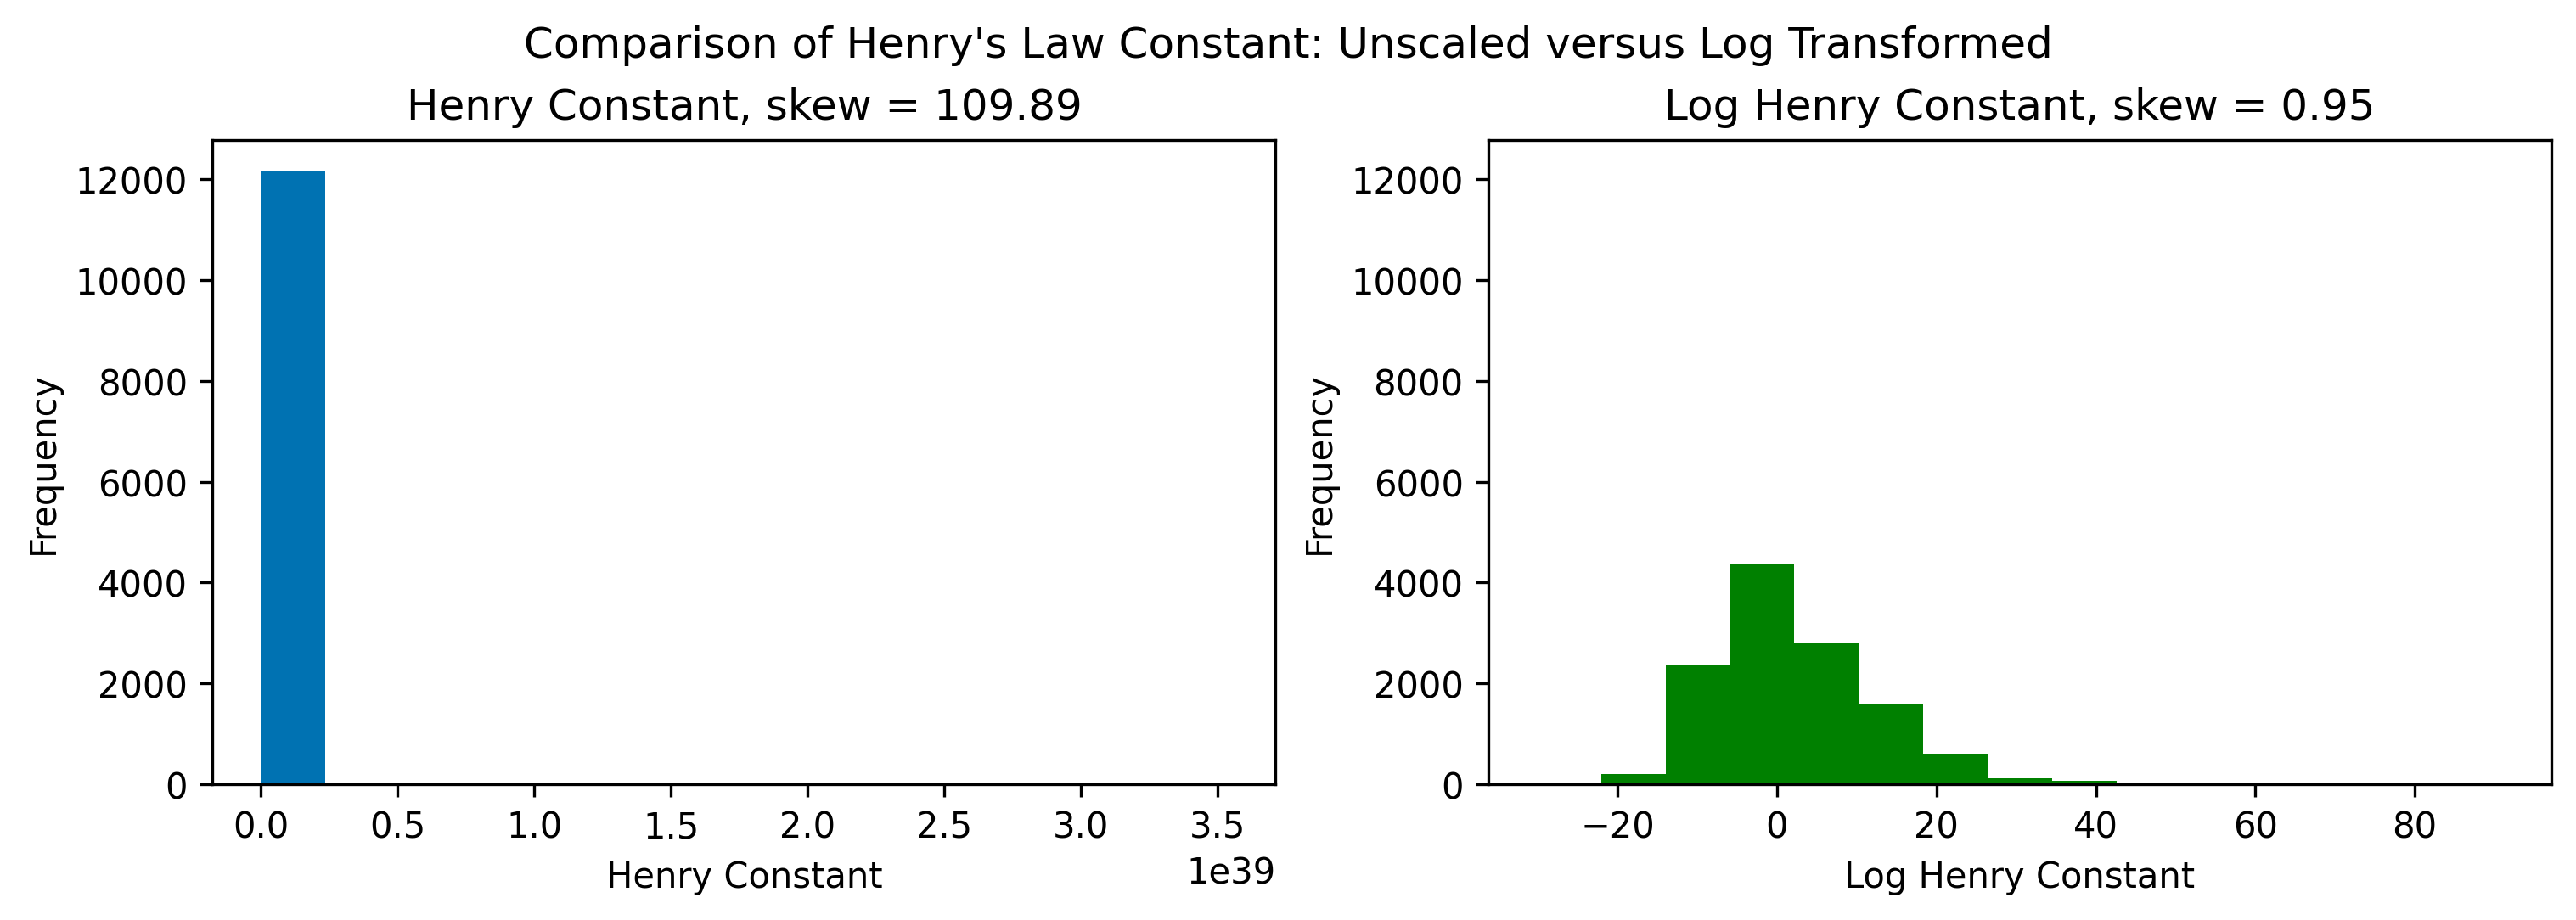
\includegraphics[width=0.9\textwidth]{figures/kH_Scaling.png}
	\caption{A comparison of distribution of values of Henry's law constant unaltered, versus log transformed.}
	\label{fig:kH_Dist}
\end{figure}

\subsubsection{Feature Engineering}
\label{subsubsec:FeatEng}
First, all missing values must be filtered out from the dataset, as the majority of machine learning algorithms cannot operate on data that contains NaNs. Next, features were scaled. 

Whilst tree-based models such as Random Forest are generally robust to lack of scaling, many others such as KNN are highly reliant on the data having the same scale\cite{KuhnJohnson}. Decreasing skew, ensuring the data lies within the same scale and removing extreme values can all help to improve a model's performance.

Each dataset was processed with functions from sklearn.preprocessing\cite{Scalers} as follows:

\begin{enumerate}
	\item If Henry's constant is the target, log transform Henry's constant and replace the raw values\footnote{The reasoning for this is explained in \ref{sec:results}}
	\item Replace $\infty$ and $-\infty$ values with NaNs
	\item Remove columns where more than 1\% of values are NaNs
	\item Remove columns where less than 1\% of values are unique
	\item Normalize features (MinMax or Normalize functions)
	\item Scale data (log1p, MaxAbsScaler, PowerTransformer, RobustScaler or StandardScaler)
	\item Outliers removed from target column ({$\log S$} or {$k_H$})
\end{enumerate}

The Z score was used as a metric to remove outliers from the target feature (e.g. $\log S$), removing anything with a score greater than 3.

\begin{equation}
Z = \frac{x - \bar{x}}{\sigma}
\end{equation}

\begin{table}[h]
	\centering
	\small

	\begin{tabularx}{0.8\linewidth}{|l|X|} %Specify table width when using tabularx otherwise IT WILL BREAK
		\hline
		\textbf{Scaling Method} & \textbf{Transformation}\\
		\hline
		MinMax & $x_{\text{std}} = \frac{x - x_{\text{min}}}{x_{\text{max}} - x_{\text{min}}}$, $y = x_{\text{std}}(x_{\text{min}} - x_{\text{max}}) + x_{\text{min}}$\cite{MinMaxScaler}\\
		Normalize & $y = \frac{x}{||x||_2}$, $||x||_2 = \sqrt{x^2_1 + x^2_2 + ... + x_n^2}$\cite{FeatEngForML}\\
		log1p & $y = \ln(1+x)$ \cite{nplog1p}\\
		MaxAbsScaler & $y = \frac{X}{|x_{\text{max}}|}$\cite{MaxAbsEq}\\

		PowerTransformer & 
		$\begin{aligned}
			y = \left\{
				\begin{array}{ll}
				\dfrac{(x + 1) ^ \lambda - 1}{\lambda}              & \lambda \neq 0, x \geq 0 \\
				\log(x + 1)                                         & \lambda =    0, x \geq 0 \\
				- \dfrac{(-x + 1) ^ {2 - \lambda} - 1}{2 - \lambda} & \lambda \neq 2, x <    0 \\
				- \log(-x + 1)                                      & \lambda =    2, x <    0
				\end{array}
			\right.
		\end{aligned}$ \cite{YeoJohnsonFEAZ, YeoJohnsonScipy}\\

		RobustScaler & $y = \frac{x_i - Q_2{x}}{Q_3(x) - Q_1{x}}$\cite{RobustEq}\\
		StandardScaler & $y = \frac{x-\mu}{\sigma}$ \cite{StandardScaler}\\
		\hline
	\end{tabularx}

	\caption{The methods used to normalise and transform the features, where $X$ is the input and $y$ is the scaled data.}
	\label{tab:scalingMethods}
\end{table}

Each scaled dataset variation was tested using the default LightGBM regressor\cite{LGBMRegressor} and a 5 fold GroupShuffleSplit with defined seed, and scores were compared to find the best scaling method. The scaling method for each dataset was chosen based on the $R^2$ score (explained later in section \ref{subsubsec:modelEvaluation}). 

A total of 2 normalisation techniques and 7 scaling methods were tested on the features, leading to a total of 15 dataset variations (14 scaling combinations and 1 unscaled). 

For both datasets, training with completely unscaled and unnormalised data gave the best results (available in section \ref{sec:Appendix}). This suggests that there are features which are naturally larger than the others, e.g. molecular weight, which could be contributing more to the model. These larger features are effectively weighted, with a greater importance compared to when normalised. When normalisation is applied, the feature no longer has this artificial weighting, and contributes less to the model, causing a reduction in score. 

Due to the importance of scaling, the best scaling method was chosen disregarding the results for the unscaled datasets.

\subsubsection{Feature Selection and Principal Component Analysis (PCA)}
\label{subsec:FeatureSelection+PCA}
\paragraph*{Feature Selection} As the data was still highly dimensional, with over 200 different features, feature selection was used to avoid the curse of dimensionality. This is the concept that the number of samples required to predict something with a given level of accuracy increases exponentially with the dimensionality of the function. This can especially become an issue for algorithms like KNN, where the number of possible neighbours increases exponentially with the number of dimensions\cite{CoD_Definition}.

With such a large number of features, many of which were sparse, it would be hard for a model to get a good representation of the population of training data without further processing. Such features that only contain 1 distinct value for all compounds will not have any overall contribution to the model\cite{CoD}.

Two different methods for feature selection were trialled: SelectKBest\cite{SelectKBest} and removing any features that have a percentage of distinct values that is lower than a given threshold. SelectKBest scores all the features using the ANOVA (Analysis of Variation) F-test, and selects the top k features, ranked by score. The F-score compares the variation between the sample means to the variation within the samples. 

By default, the scoring function was set to 'f\_classif' and this was not changed. This function calculates the F-score. This choice in scoring function was likely a contributing factor to its poor performance (table \ref{tab:SelectKBest}), where using the maximum number of features gave the best results, even when many of those features only contained a singular value. Ideally, this should have been changed to a regression scorer, such as `f\_regression'. The equations\cite{fstat} for 'f\_classif' are given below (sample frequency, followed by F-score):

\begin{align}
	s^2 &= \frac{\sum(x-\bar{x})^2}{(n-1) \label{eq:sampleFreq}}\\
	F &= \frac{s^2_a}{s^2_b} \label{eq:fscore}
\end{align}

The final method that was trialled, and later chosen, for feature selection was based off calculating the percentage of values in the column that were unique, and dropping any columns where this percentage was below a given threshold (1\%). This proved to be the most effective and straightforward to use, since it was not reliant on a more complex equation or statistical test.

\begin{equation}
	\text{Percentage Unique} = \frac{\text{Number of Unique Values}}{\text{Total Number of Values}} \times 100
\end{equation}

\begin{figure}[H]
	\centering
	\small
	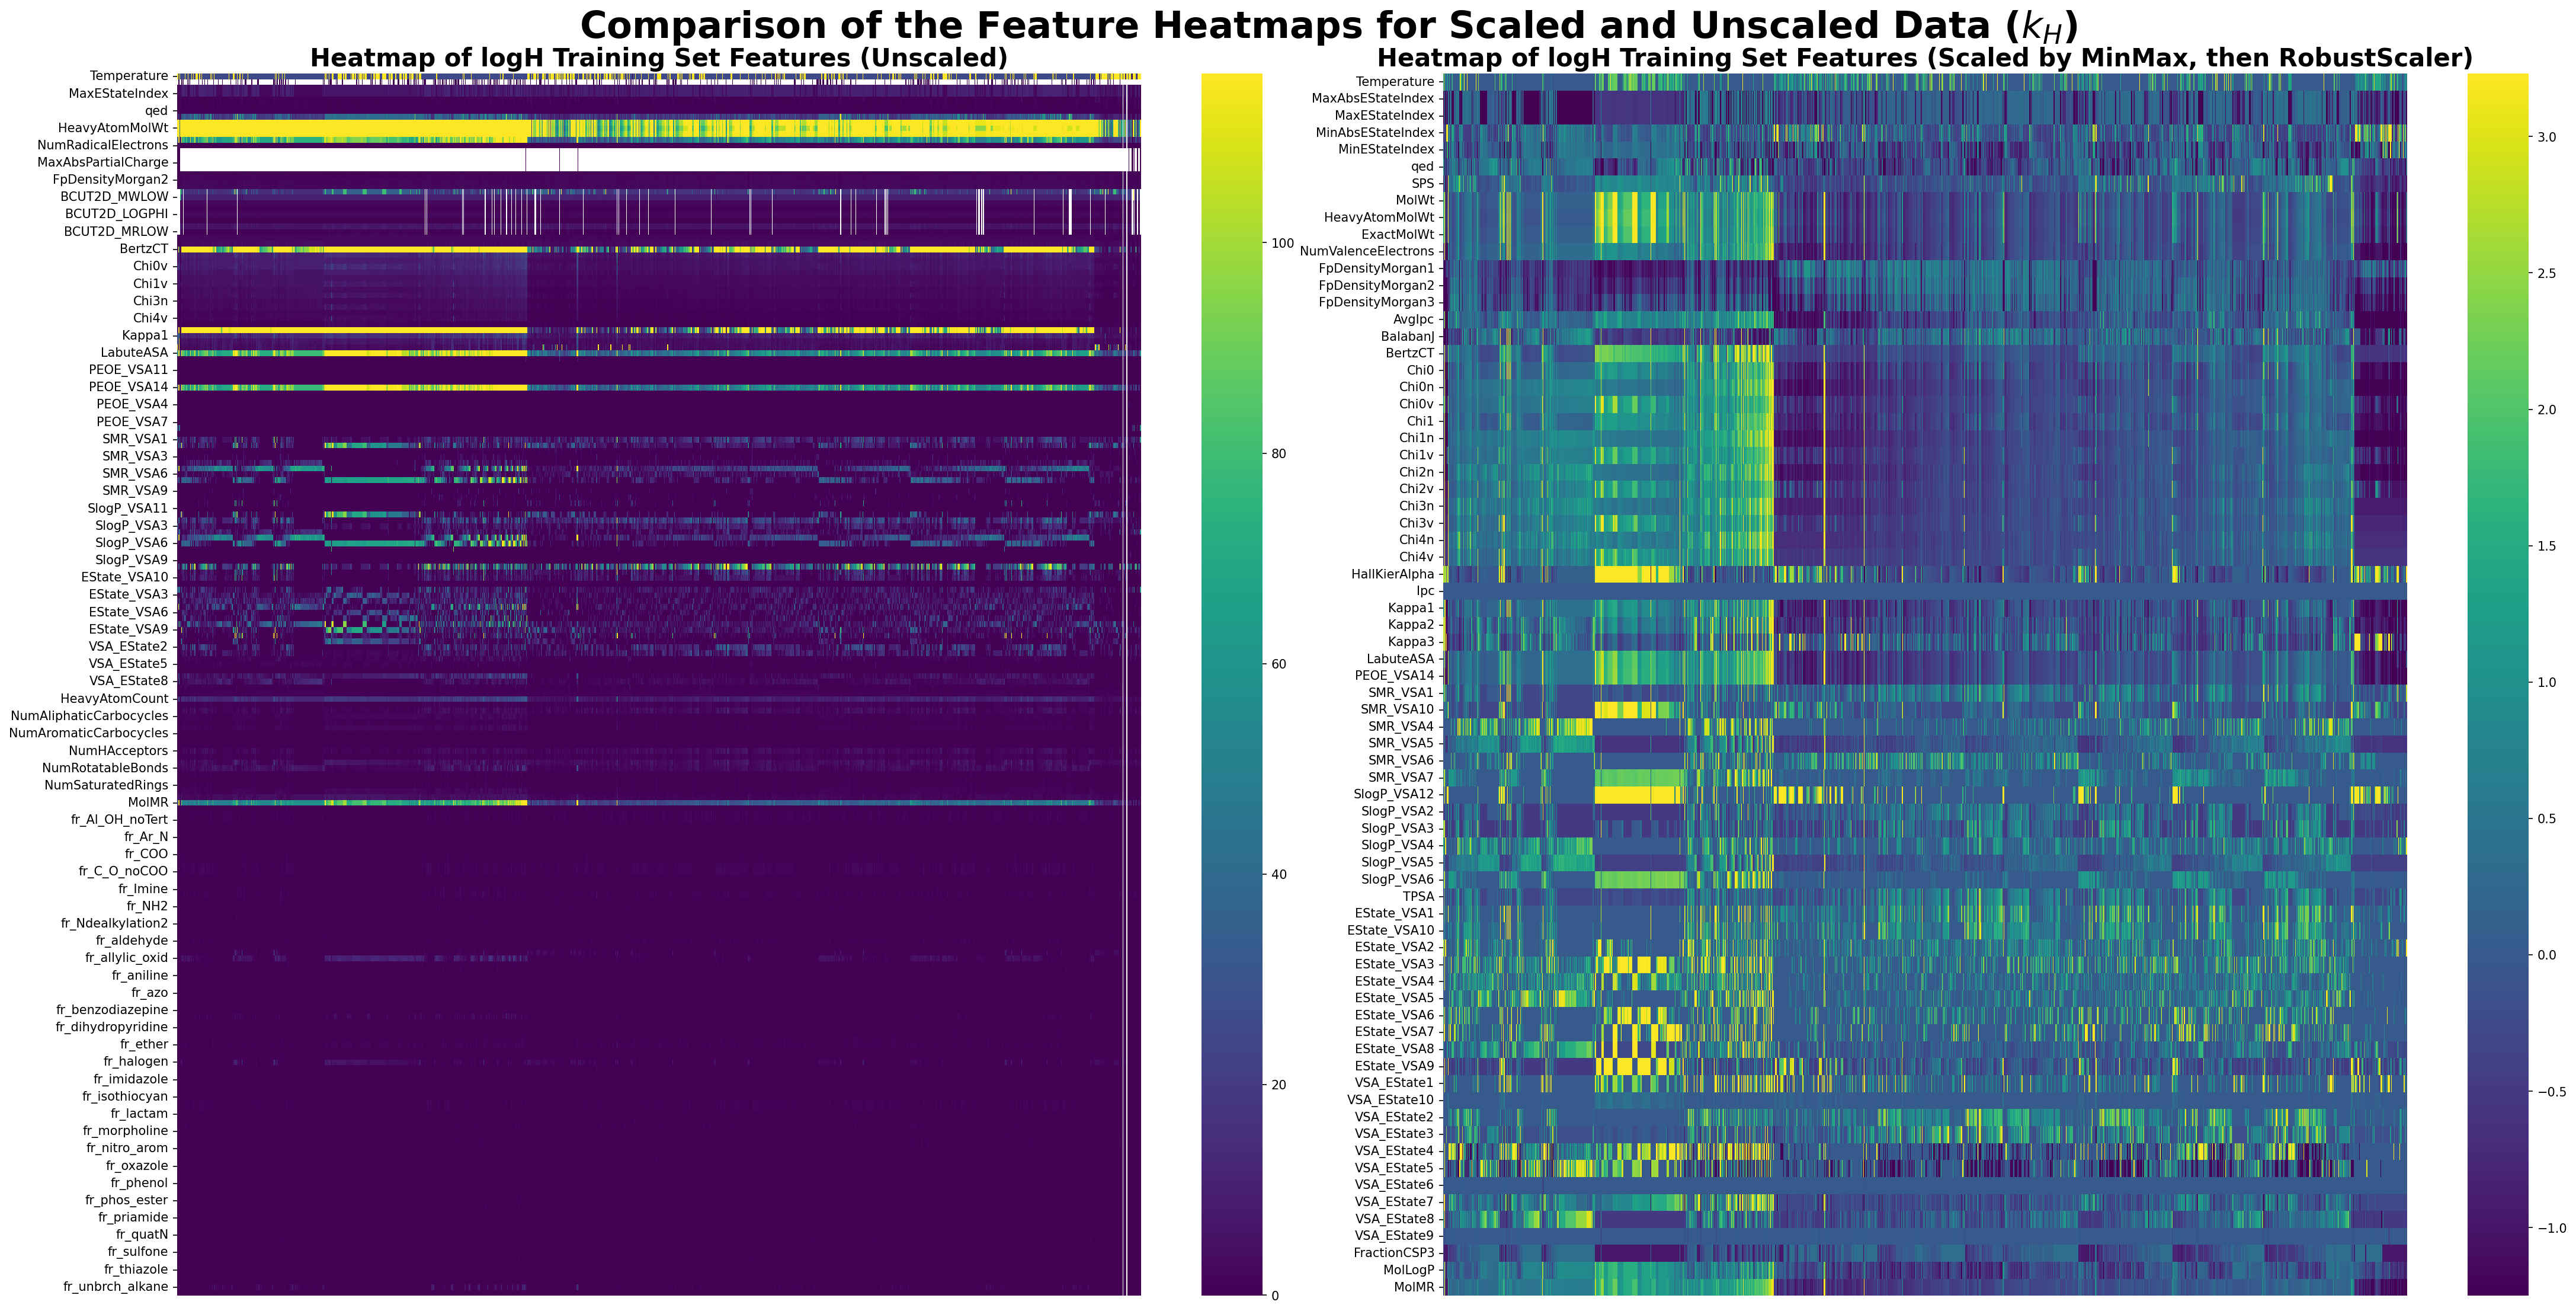
\includegraphics[width=0.9\textwidth]{figures/HeatmapScalingComparison.png}
	\caption{A heat-map comparison of the $\log k_H$ dataset before and after scaling and feature selection.}
	\label{fig:HeatmapScalingComparison}
\end{figure}

Fig. \ref{fig:HeatmapScalingComparison} displays the difference in the data distribution before and after scaling. There are no longer missing values in the dataset, and the overall range of values is smaller, yet there is more distinction between them. Additionally, all the features are now on the same scale.

\paragraph*{Principal Component Analysis (PCA)} The sklearn implementations of Kernel PCA\cite{KernelPCA} and standard PCA\cite{PCA} were tested across a range of components from 1 to the total number of features. PCA is an unsupervised method of dimensionality reduction in which features that are linearly dependent, or correlated, are reduced into a lower dimensional linear subspace. It attempts to maintain as much relevant information as possible. However, it assumes that data with low variance is unimportant; in this way, it is not suitable for all datasets and models\cite{PCA_IBM, PCA_UCL, FeatEngForML}.

Kernel PCA is a variant of PCA that is designed to deal with non-linearity in data\cite{KernelPCAPaper}. Using kernels can sometimes handle complex data better than only using Euclidean distances\cite{KPCA_Alt_Paper}. It was trialled after standard PCA was found to have a highly detrimental effect on model performance, reducing the $R^2$ by 0.5 or more (results available in appendix \ref{subsec:PCA_Results}). 

A variety of different kernels were trialled, using a bisection algorithm to determine the highest $R^2$ output with a given number of components. However, the best number of components was consistently the total number of features in the dataset, and it still yielded worse scores than using no PCA or kernel PCA whatsoever. For this reason, PCA was ultimately discarded.

\subsection{Machine Learning}
\label{subsec:ML}
\subsubsection{Algorithms}
\label{subsubsec:Algorithms}
The No Free Lunch Theorem\cite{NoFreeLunch} approach was taken for deciding on which algorithms to use. After determining the best scaling method for the data, 7 different regression algorithms were trialled\footnote{A neural network\cite{pytorch} was also tested but removed due to time constraints.}. Each algorithm and scaling pair was optimized using a parameter grid search, with the sklearn function GridSearchCV\cite{GridSearchCV}. Post-optimization, each model was run again with a 5 fold GridShuffleSearch, and scored with MSE and $R^2$. The model for each dataset with the highest $R^2$ and lowest MSE was used to make the final predictions.

\begin{table}[H]
	\begin{minipage}{.5\linewidth}
		\centering
		\small
		\begin{tabular}{|l|c|c|}
			\hline
			\textbf{Algorithm} & \textbf{MSE} & $\mathbf{R^2}$\\
			\hline
			\textbf{LightGBM} & \textbf{1.01} & \textbf{0.80} \\
			Kernel Ridge Regression & 1.06 & 0.79 \\
			KNN & 1.23 & 0.76 \\
			Random Forest & 1.28 & 0.75 \\
			AdaBoost & 1.53 & 0.70 \\
			Support Vector Regression & 1.65 & 0.68\\
			\hline
		\end{tabular}
		\caption{Algorithm testing on v0.6.0 version of the $\log S$ dataset.}
		\label{tab:AlgLogS}
	\end{minipage}
	\begin{minipage}{.5\linewidth}
		\centering
		\small
		\begin{tabular}{|l|c|c|}
			\hline
			\textbf{Algorithm} & \textbf{MSE} & $\mathbf{R^2}$\\
			\hline
			\textbf{LightGBM}  & \textbf{5.04}& \textbf{0.89} \\
			Kernel Ridge Regression & 5.92	  & 0.87		  \\
			Random Forest	   & 8.74		  & 0.81		  \\
			KNN & 9.31		  & 0.81		  \\
			AdaBoost		   & 0.73		  & 0.73		  \\
			Support Vector Regression & 68.92 & -0.45		  \\
			\hline
		\end{tabular}
		\caption{Algorithm testing on v0.6.0 version of the $\log k_H$ dataset.}
		\label{tab:AlgLogH}
	\end{minipage}
\end{table}

Hyperparameters are available in the appendix, section \ref{subsec:ModelHyperparameters}.
\paragraph*{Ensemble Methods}
Ensemble methods are algorithms that aggregates a set of models (regressors or classifiers) on a subset of the training data, then train further models using a weighted vote or average of their predictions\cite{EnsembleMethods}. This method relies on the idea that a collection of models, or learners, has a greater overall accuracy than a single model. They tend to avoid overfitting, and are not as affected by the curse of dimensionality as other methods\cite{Ensemble_IBM}, like support vector regression. Two types of ensemble learning methods were trialled: Gradient Boosting and Random Forest.

Multiple different variations of gradient boosting exist. Here, the AdaBoost and the LightGBM regressor gradient boosting algorithms were chosen. Gradient boosting is an iterative method in which a sample of data is selected, a set of models are trained on it, and the next iteration of models attempts to learn from its predecessors using the residuals. Models are trained sequentially, sampling with replacement from the training set\cite{Boosting_IBM}. Using this method, some models may perform significantly better on some parts of the dataset but worse on others, but when aggregated, give a much better result overall.

\begin{description}
	\item \textbf{Adaboost}\quad AdaBoost is a type of gradient boosting regressor that varies from standard boosting methods in that it is adaptive, hence the name. Instead of the new models learning from the previous ones, the worst scoring predictions have their selection probability increased so they are more likely to appear in the next iteration of the training set. In other words, the weight of the worst scoring datapoints is adjusted. This weighting is what separates AdaBoost from standard boosting algorithms\cite{AdaBoostDrucker}.
	%
	\item \textbf{LightGBM Regressor}\quad The LightGBM boosting regressor is a variant of the Gradient Boosting Decision Tree algorithm that uses a combination of Gradient-based One-Side Sampling and Exclusive Feature Bundling, which together decrease the training time compared to a traditional gradient boosting algorithm by `up to over 20 times`\cite{LightGBMPaper}. This model was chosen for testing due to its previous performance in models relating to miscibility. 
	%
	\item \textbf{Random Forest Regressor}\quad The LightGBM implementation of the Random Forest regressor was used\cite{LGBMRegressor}. This algorithm is a type of regressor, containing a collection of tree-structured classifiers $\left\{h(\mathbf{x}, \Theta_k), k=1,\dots\right\}$ that depend on a random vector $\Theta$ so that the tree predictor $h(\mathbf{x}, \Theta)$, has numerical values instead of classes. 
	
	It is noted that the type of randomness used in this algorithm may be more suitable for classification problems than regression, however the Random Forest algorithm cannot overfit due to the Law of Large Numbers\cite{Breiman2001}.
\end{description}

\paragraph*{Single Models}
\begin{description}
	\item \textbf{Support Vector Regression (SVR)}\quad The sklearn implementation (based on libsvm\cite{libsvm}) of SVR\cite{SupportVectorRegression} was used in this project. A Support Vector Regression model is a generalisation of a Support Vector Machine, with the introduction of an $\epsilon$ tube, where $\epsilon$ is the tolerance margin. The support vectors are defined as any points which lie outside of the $\epsilon$ tube - the larger $\epsilon$ is, the more support vectors there are. SVR is different to other algorithms in that it uses a symmetrical loss function, measuring the absolute loss\cite{Awad2015}.
	
	Some of the key advantages of this algorithm is that it is said to be good at generalisation, and have high precision/accuracy. Conversely, one of the disadvantages of this algorithm implementation in particular is its high fit time complexity (more than quadratic), which means it took a long time to train each model. It relies on kernel functions, and aims to find a function that fits the target with an error of no greater than the  $\epsilon$ tube width for each target datapoint. The algorithm iterates until a specified convergence criterion is met\cite{SVR_MathWorks}. 
	%
	\item \textbf{Kernel Ridge Regression}\quad Kernel Ridge Regression is a variant of Support Vector Regression that uses a squared error loss instead of $\epsilon$-insensitive loss\cite{KRR_Scikit}. It replaces all datapoints with their feature vector (eq. \ref{eq:featVec}), which can cause the number of dimensions to increase infinitely higher than the number of datapoints\cite{KRR_Welling}. The kernel trick is then used to process the data without having to complete a calculation for every feature vector\cite{KRR_Haugh}. The kernel trick is the application of a kernel function, e.g. the sigmoid kernel, to data to transform it to a higher dimensional space\cite{IBM_SVM}. This is followed by performing computations on it within that higher dimensional space, yet without having to do an infinite amount of work.

	\begin{equation}
		\mathbf{x}_i \rightarrow \Phi_i = \Phi(\mathbf{x}_i)
		\label{eq:featVec}
	\end{equation}
	%
	\item \textbf{K-Nearest Neighbour Regressor (KNN)}\quad KNN is an algorithm that is most often used for classification problems. It assumes that like datapoints are close to one another using a given space metric, e.g. Euclidean, or Manhattan. It is a type of 'lazy learning' method, which can be quite memory intensive depending on the size of the dataset used. Despite its simplicity to implement, it is prone to issues such as the curse of dimensionality and overfitting\cite{KNN_IBM}.
	%
	\item \textbf{Linear Regression}\quad A linear regression is one of the simplest possible machine learning algorithms. It fits a line of best fit to the targets, and minimises the residual sum of squares between the target value and the predicted value\cite{LinearRegression}. Linear regression was only used on the first version of the dataset and not continued further due to results. 
\end{description}

\subsubsection{Model Training}
\label{subsubsec:modelTraining}
\paragraph*{Preliminary Testing}
The full dataset for each target variable was separated into a training set and a validation set, with a randomly generated 85:15 split by InChI. Models were trained and tested on the training set using a variation of KFold, GroupShuffleSplit\cite{GroupShuffleSplit}, with 5 folds. GroupShuffleSplit splits the dataset based on a group, InChI, rather than solely by target variable like standard KFold. Using this method ensured that a compound could not appear in both the training and test set, minimising data leakage. By iterating through the folds, a prediction was made for every entry in the training set. This method was used for determining what algorithm and what scaling method to use.

\paragraph*{Obtaining Results}
The dataset containing both {$\log S$} and {$k_H$} was used as the test set. The {$\log S$} dataset was used as the training set for {$\log S$}, and used as the prediction set for {$k_H$}, and vice versa for the Henry's constant set. 
\begin{table}[H]
    \centering
    \small
    \begin{tabularx}{\linewidth}{|l|X|}
        \hline
        \textbf{Dataset} & \textbf{Usage} \\
        \hline
        Henry's constant & Training Henry's law model, prediction set for missing {$\log S$} values \\
        $\log S$ & Training {$\log S$} model, prediction set for missing Henry's constant values \\
        Henry's constant and {$\log S$} & Test set for both models \\
        \hline
    \end{tabularx}
    \caption{Datasets used to obtain the results and create the final output dataset.}
    \label{tab:PredSets}
\end{table}

The datasets were scaled according using the best scoring scaling method (MinMax $\rightarrow$ RobustScaler for both), and the best scoring algorithm was trained and used to predict the missing values. The predicted values were added to a copy of the Cleaned Master dataset and the data source columns were updated accordingly. Henry's law constant was also unscaled.

Additionally, predictions were also made for the test set, and metrics were calculated and used to evaluate overall model performance.

\subsubsection{Model Evaluation}
\label{subsubsec:modelEvaluation}
Models were evaluated based on $R^2$ and Mean Squared Error (MSE). %following text is lifted from paper. Need to check if that's ok

Mean Squared Error:\\ 
\begin{equation}
    \text{MSE} = \frac{\Sigma(y_{i}-\hat{y}_{i})^{2}}{n}
    \label{eq:mse}
\end{equation}
Mean squared error is a metric of the Euclidean distance between the predicted y value and the true y value. The greater the error, the more inaccurate the model is.\\
\newline
$R^{2}$ Score (Coefficient of Determination):\\
\begin{equation}
    R^{2} = 1 - \frac{\Sigma_{i}(y_{i} - \hat{y_{i}})^{2}}{\Sigma_{i}(y_{i}-\bar{y})^{2}}
    \label{eq:r2}
\end{equation}
The $R^{2}$ score measures how well the predicted y values and the true y values correlate to each other.\cite{r2} A perfect correlation would have an $R^{2}$ value of $1$, no correlation scores $0$, and perfect negative correlation would be $-1$. 

One of the key disadvantages of both these metrics is that they are very easily skewed by extreme values. In particular, the presence of a few points can cause a large increase in $R^{2}$. Additionally, $R^{2}$ values tend to be higher when there is a large amount of variance in the values it is comparing\cite{KuhnJohnson}.

\section{Results and Analysis}
\label{sec:results}
\subsection{Final Predictions}
\label{subsec:FinalPreds}
\subsubsection{Solubility}
\begin{figure}[H]
	\centering
	\small
	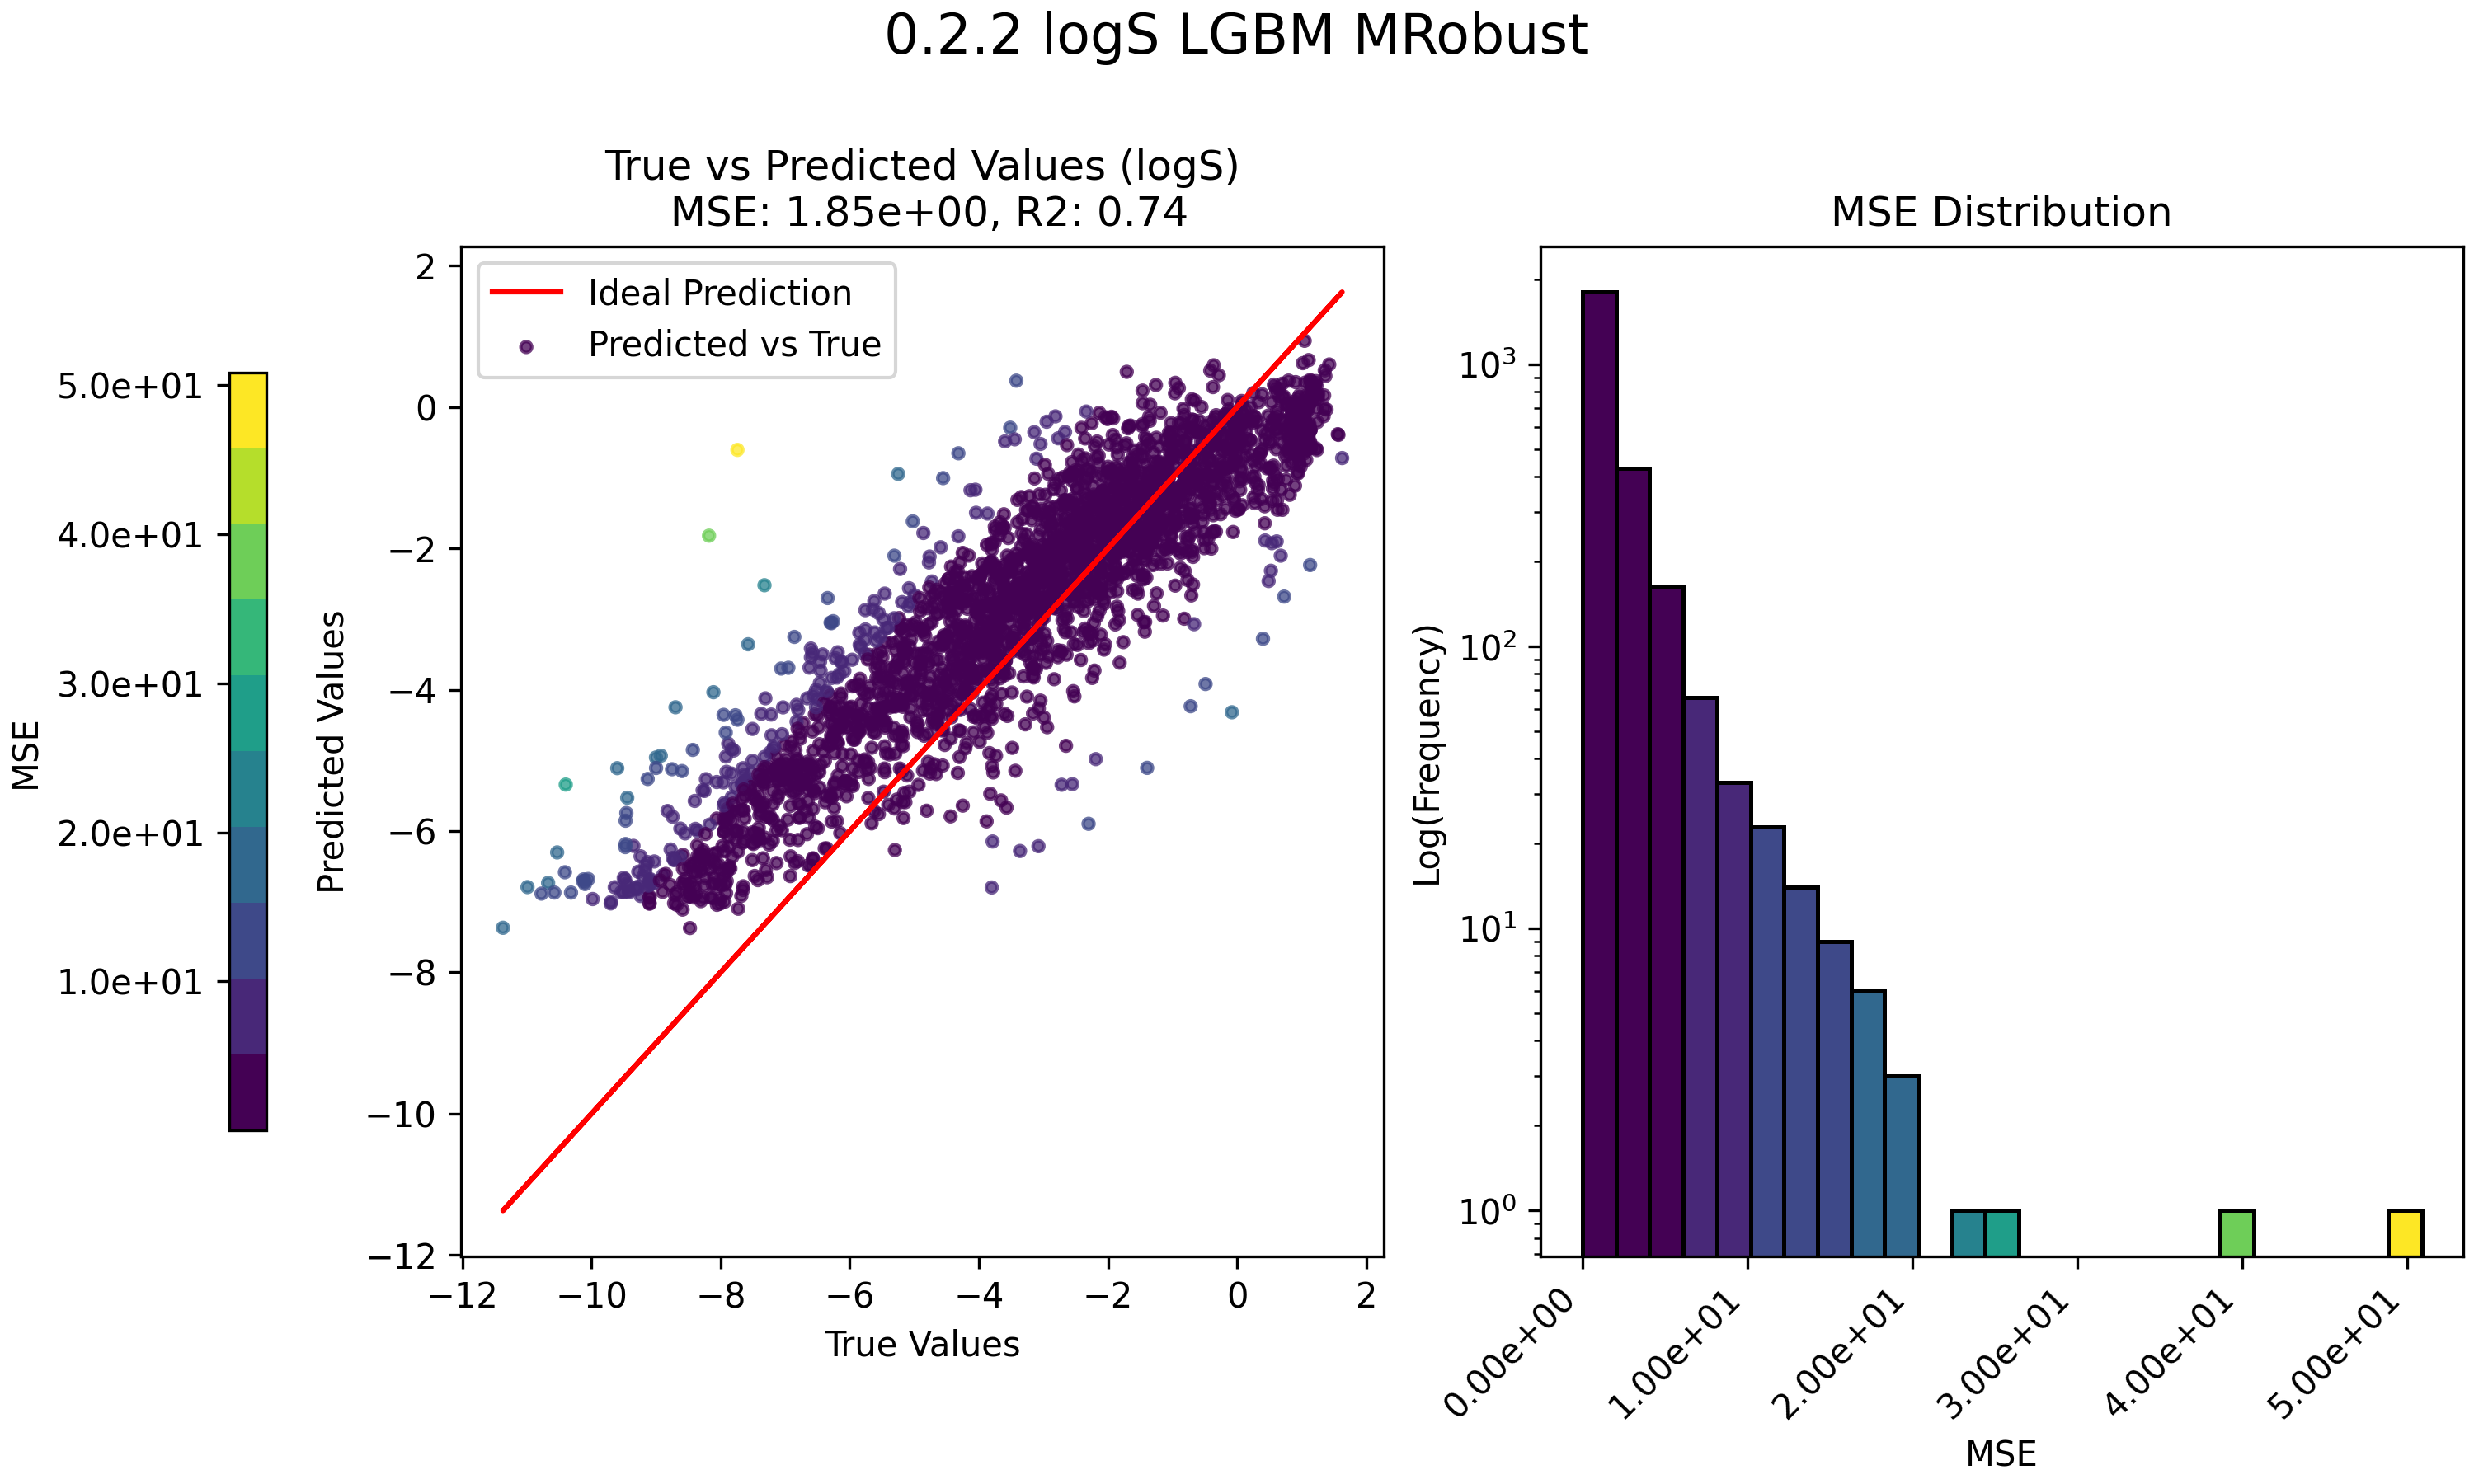
\includegraphics[width=0.8\linewidth]{figures/0.2.2-PredLogS.png}
	\caption{From left to right: the scatter plot of true versus predicted {$\log S$} values for the test set (v0.2.2), and the distribution of the associated MSE for each prediction}
	\label{fig:PredLogS}
\end{figure}

\begin{table}[H]
	\centering
	\small
	\begin{tabular}{|l|c|}
		\hline
		\textbf{Metric} & $\log S$\\
		\hline
		$\mathbf{R^2}$ & 0.73 \\
		\textbf{MSE} & 1.85 \\
		\textbf{\% MSE $>$ 1} & 45.52\% \\
		\hline
	\end{tabular}
	\caption{The final scores for the {$\log S$} test set (v0.2.2) predictions}
	\label{tab:logS_Scores}
\end{table}
Overall, the model to predict solubility performed well, consistently obtaining a moderately low MSE and a high $R^2$ score. In the later versions of the dataset, the scores worsen in comparison to earlier iterations, e.g. $R^2 = 0.84$ in table \ref{tab:ScalingLogS} with v0.4.2 of the dataset. This is likely due to changes in the distribution of data in the dataset as more datapoints were added, and data processing methods were adjusted and debugged. It is likely that scores would improve again if hyper-parameter optimization was performed again to reflect the changes in the data. 

In terms of error by compound, it appears that the vast majority of compounds were predicted well (note that the y-axis is log scaled in the histogram in Fig. \ref{fig:PredLogS}), with a few major outliers. 

\begin{figure}[H]
	\begin{minipage}{0.5\linewidth}
		\centering
		\small
		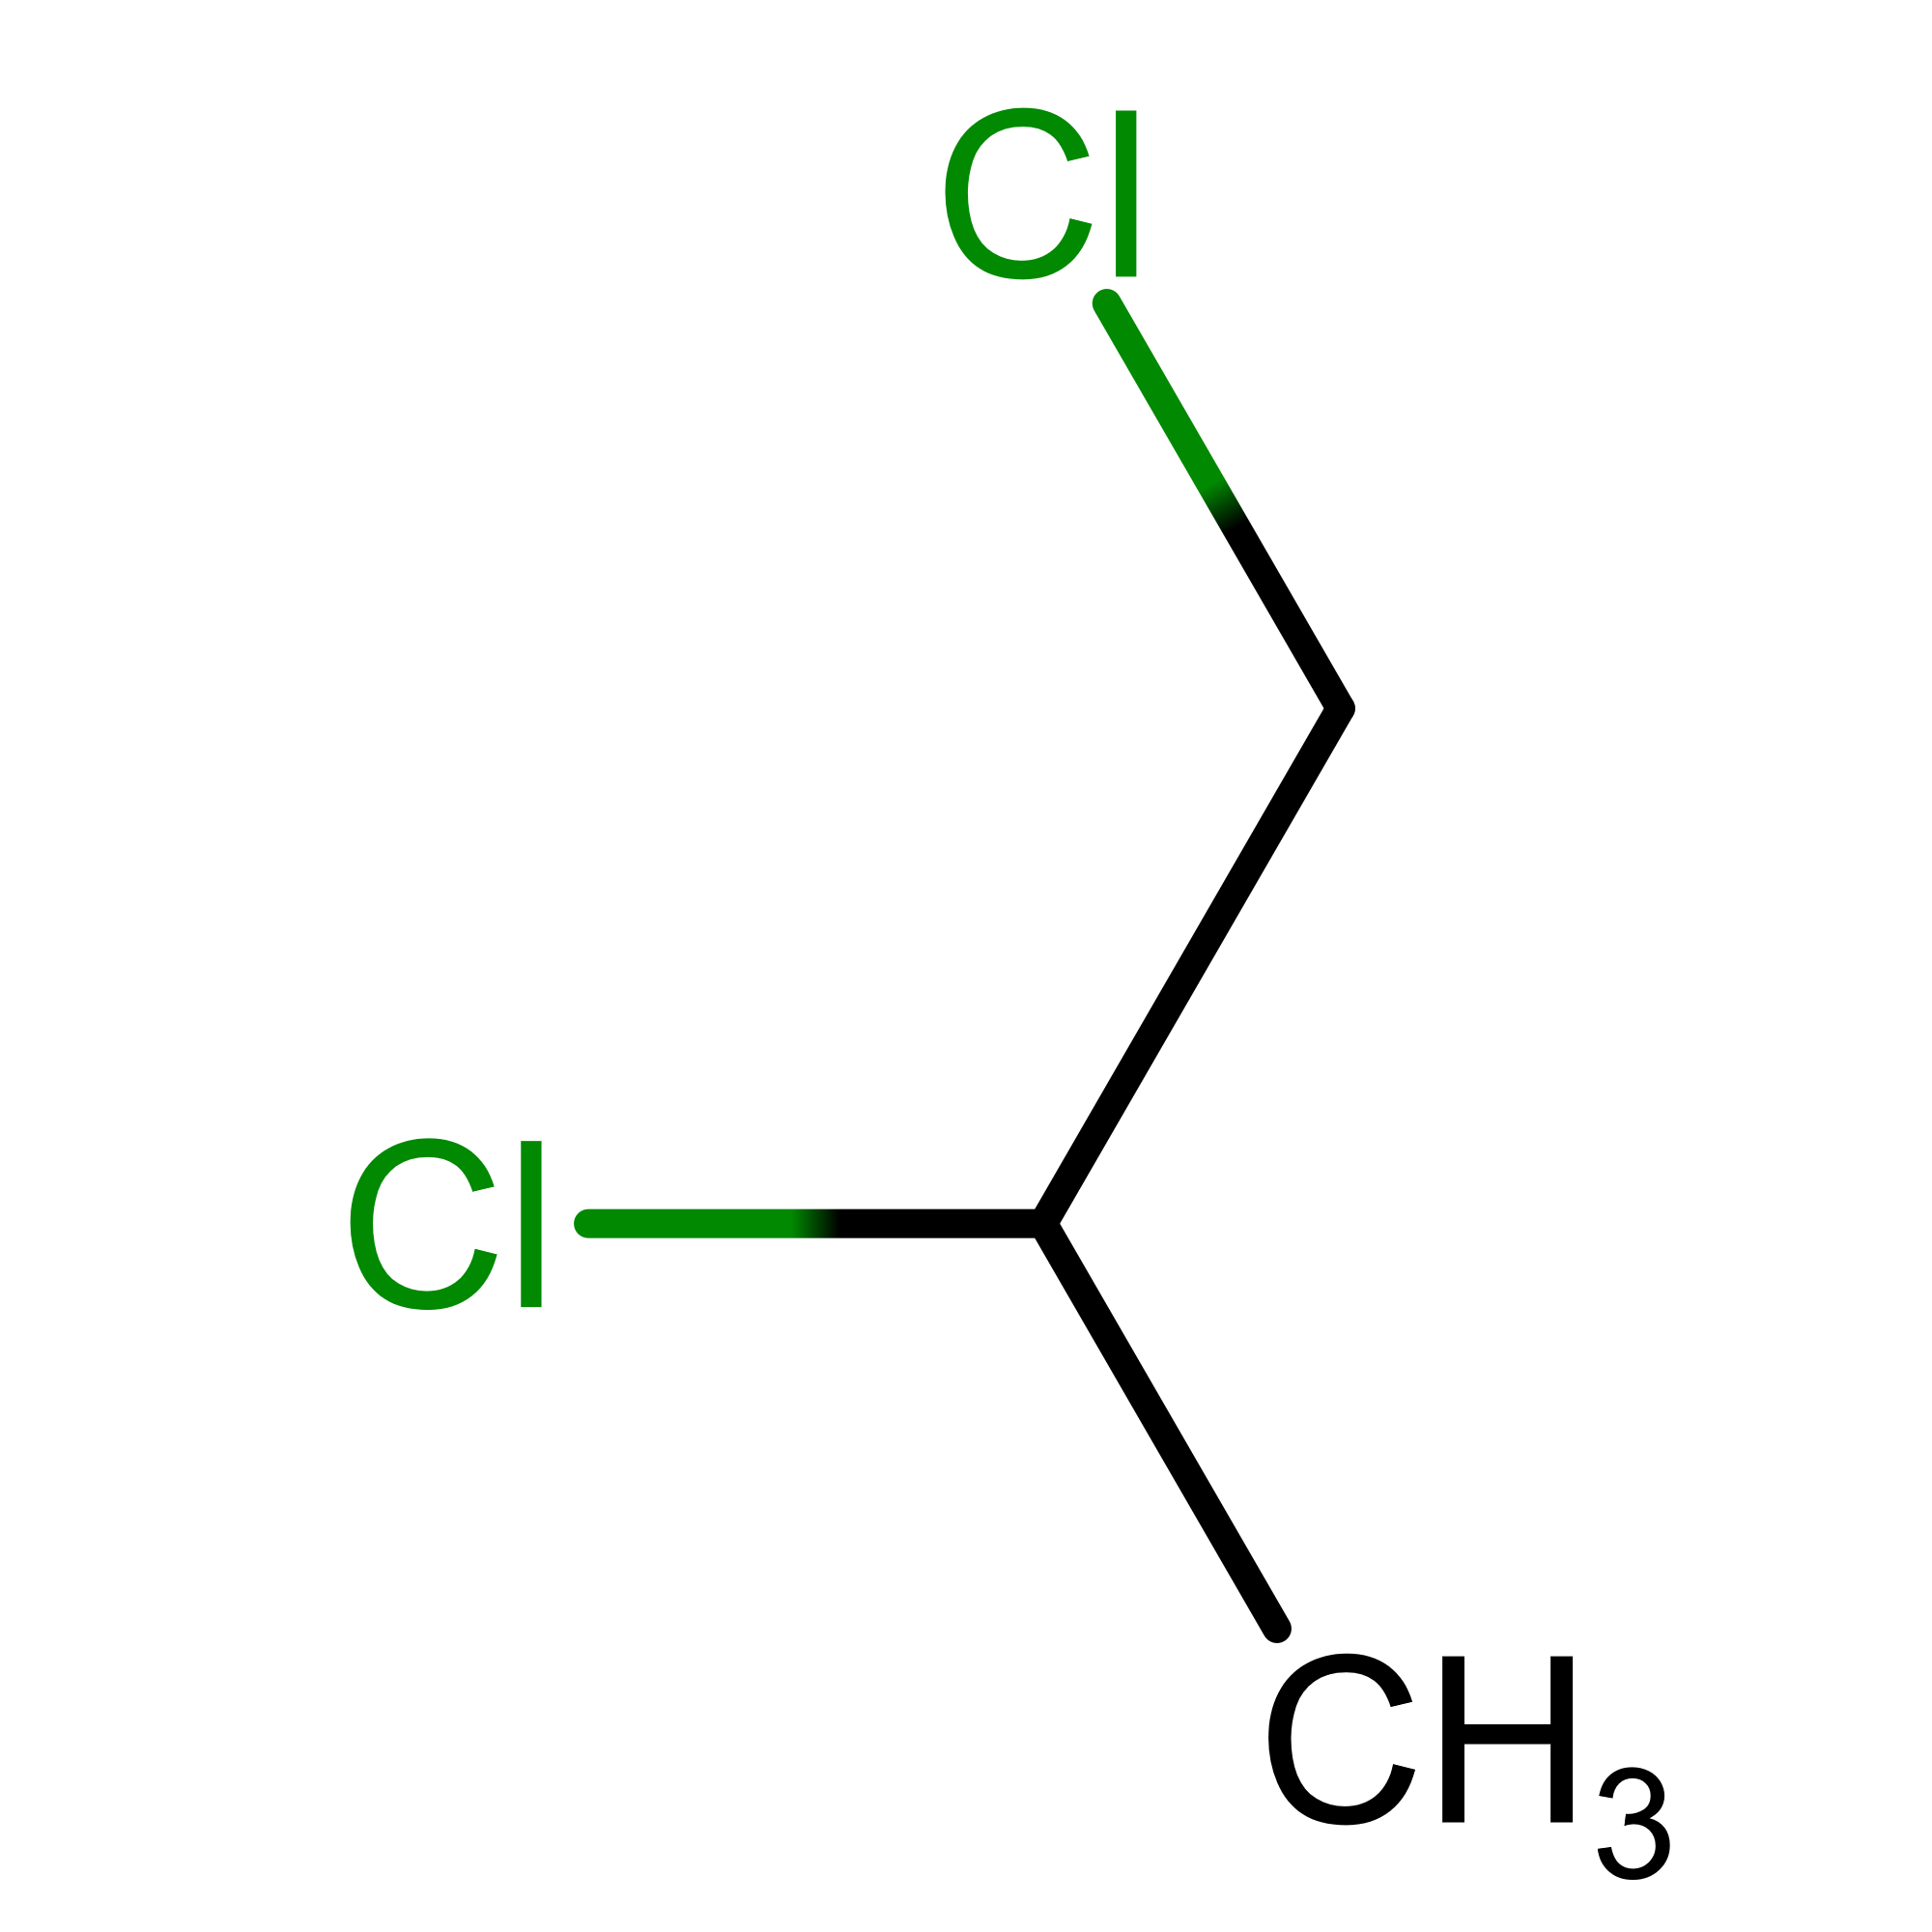
\includegraphics[width = 0.5\linewidth]{figures/logSWorst.png}
		\caption{The least accurately predicted compound, 1,2-dichloropropane\cite{WorstLogSName},  in the $\log S$ test set (MSE = 50.87)}
		\label{fig:WorstLogS}
	\end{minipage}
	\begin{minipage}{0.5\linewidth}
		\centering
		\small
		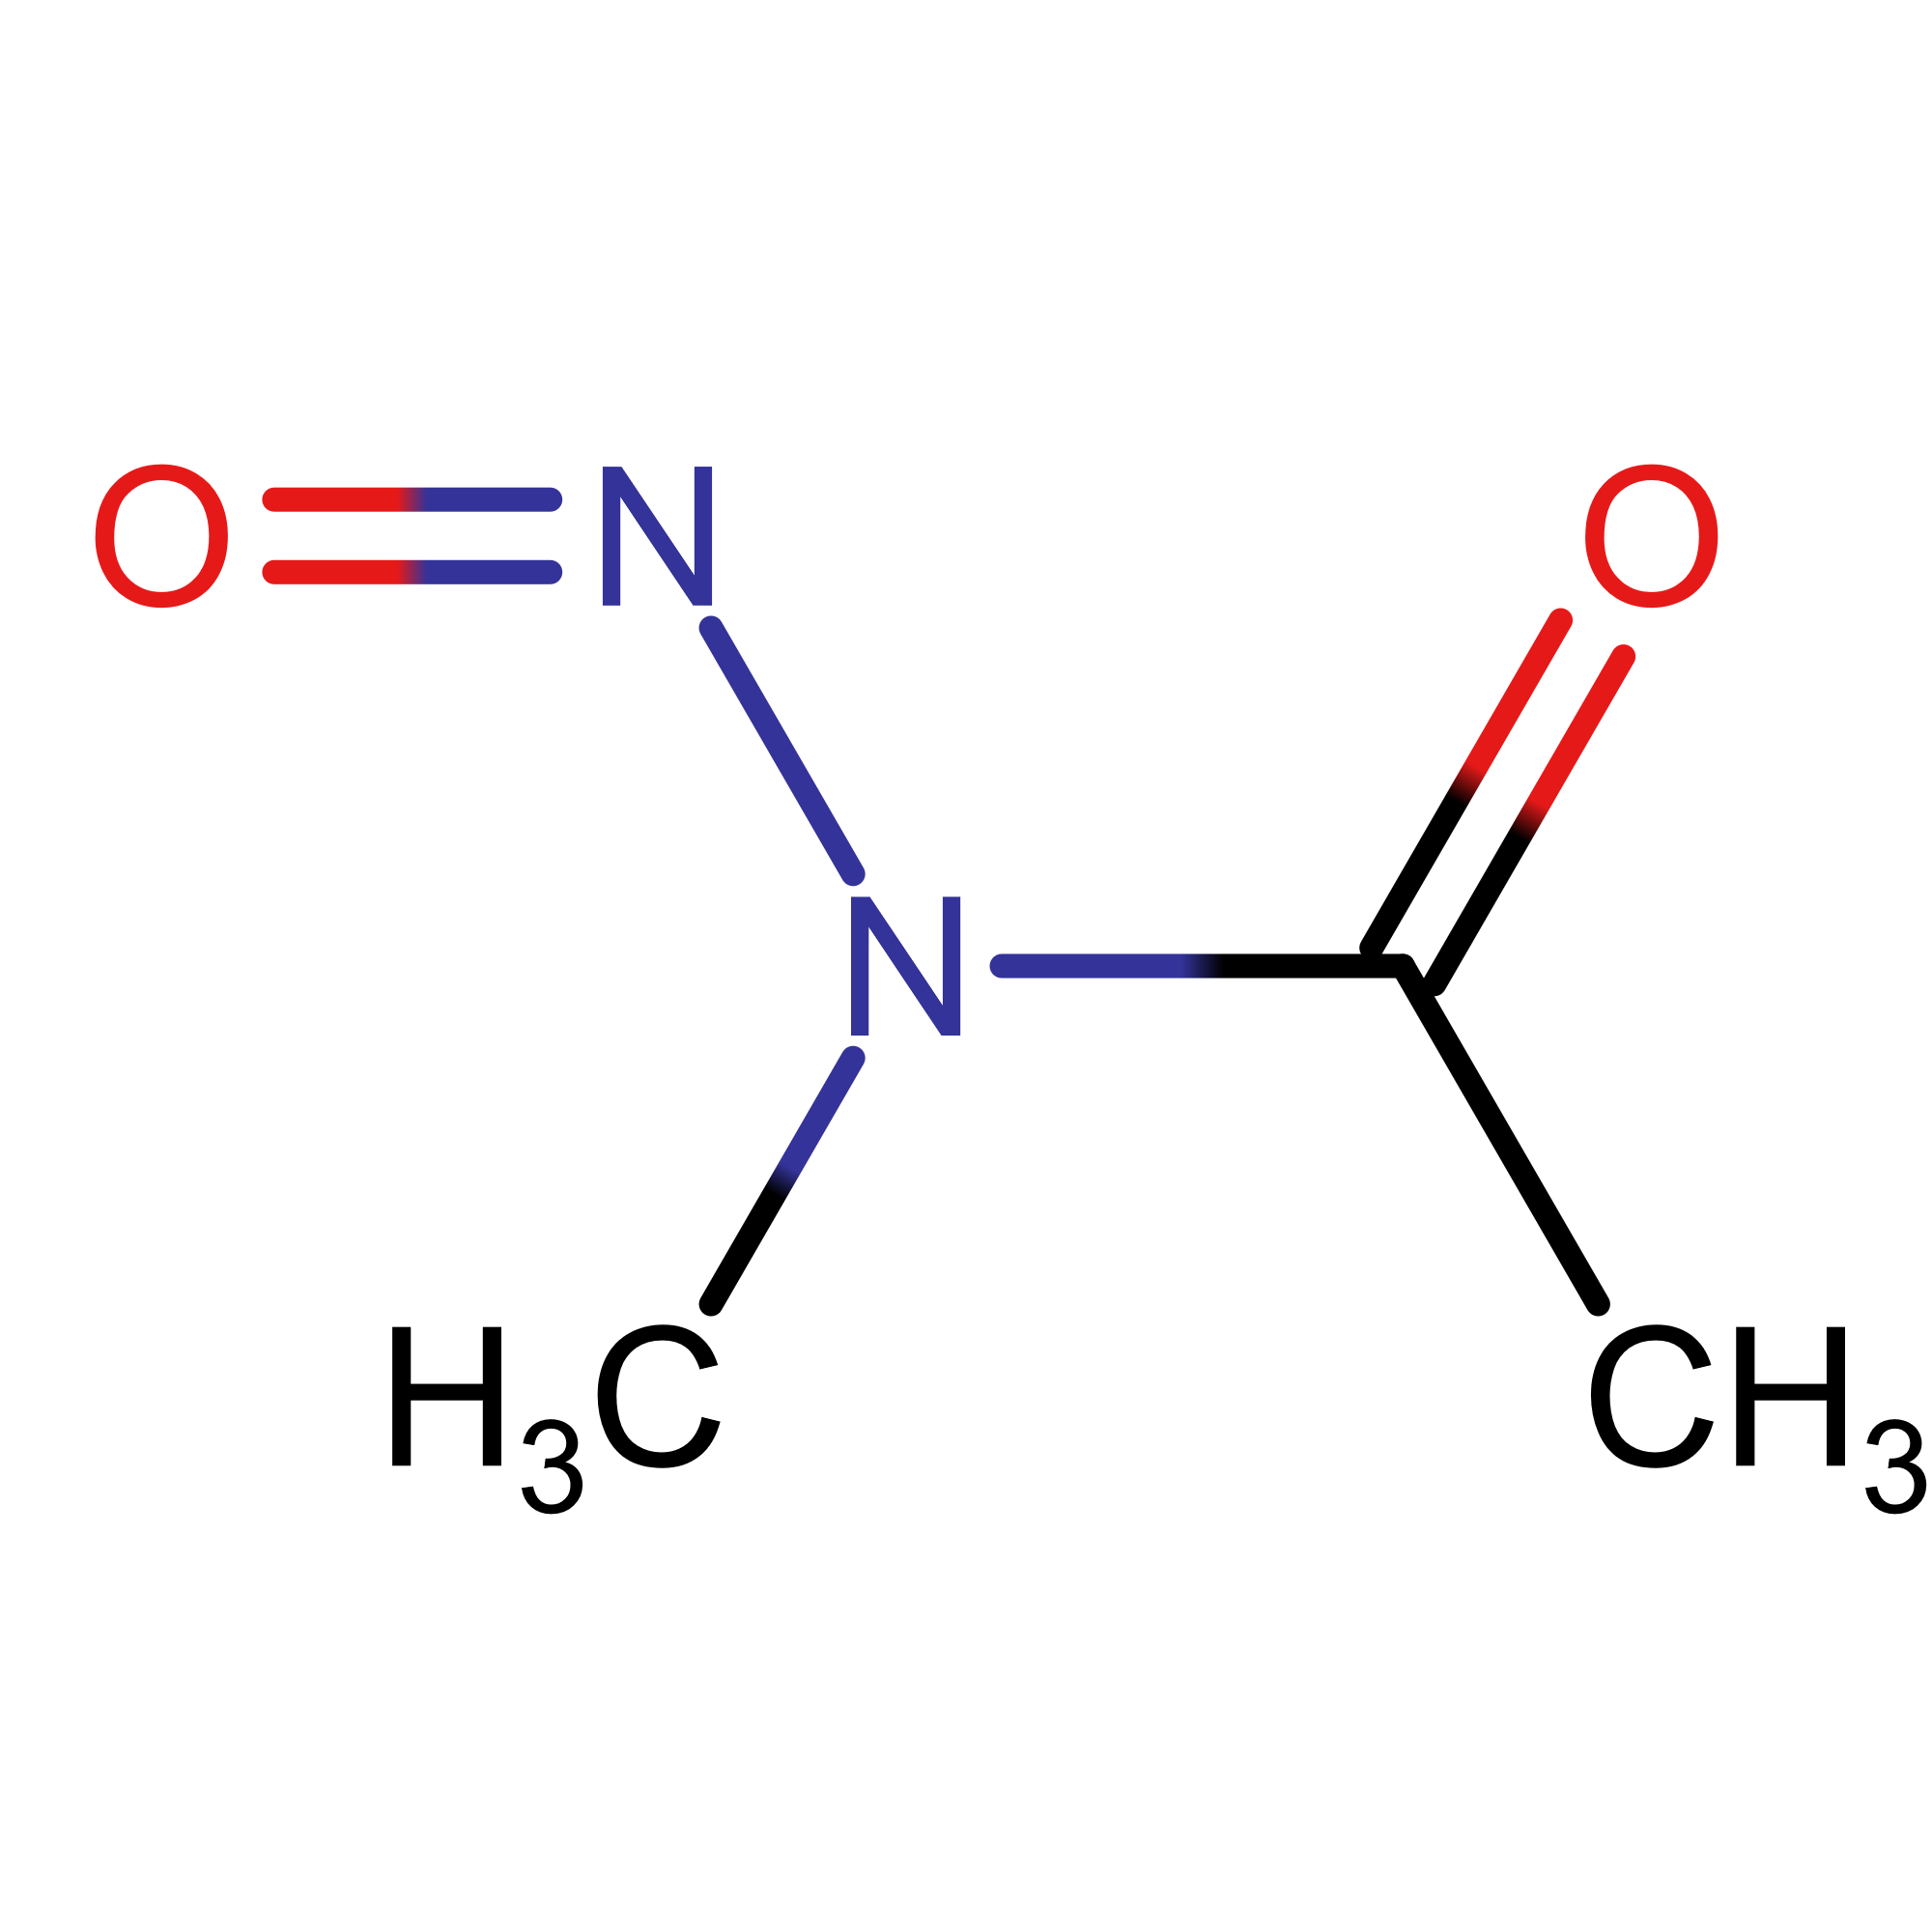
\includegraphics[width = 0.5\linewidth]{figures/logSBest.png}
		\caption{The most accurately predicted compound, N-Methyl-N-nitrosoacetamide\cite{WorstLogSName},  in the $\log S$ test set (MSE = 6.01e-07)}
		\label{fig:BestLogS}
	\end{minipage}
\end{figure}

Currently, it is unknown why these compounds in particular were handled particularly well or badly by the model. This is something to be explored in the future.

\subsubsection{Henry's law constant}
\begin{figure}[H]
	\centering
	\small
	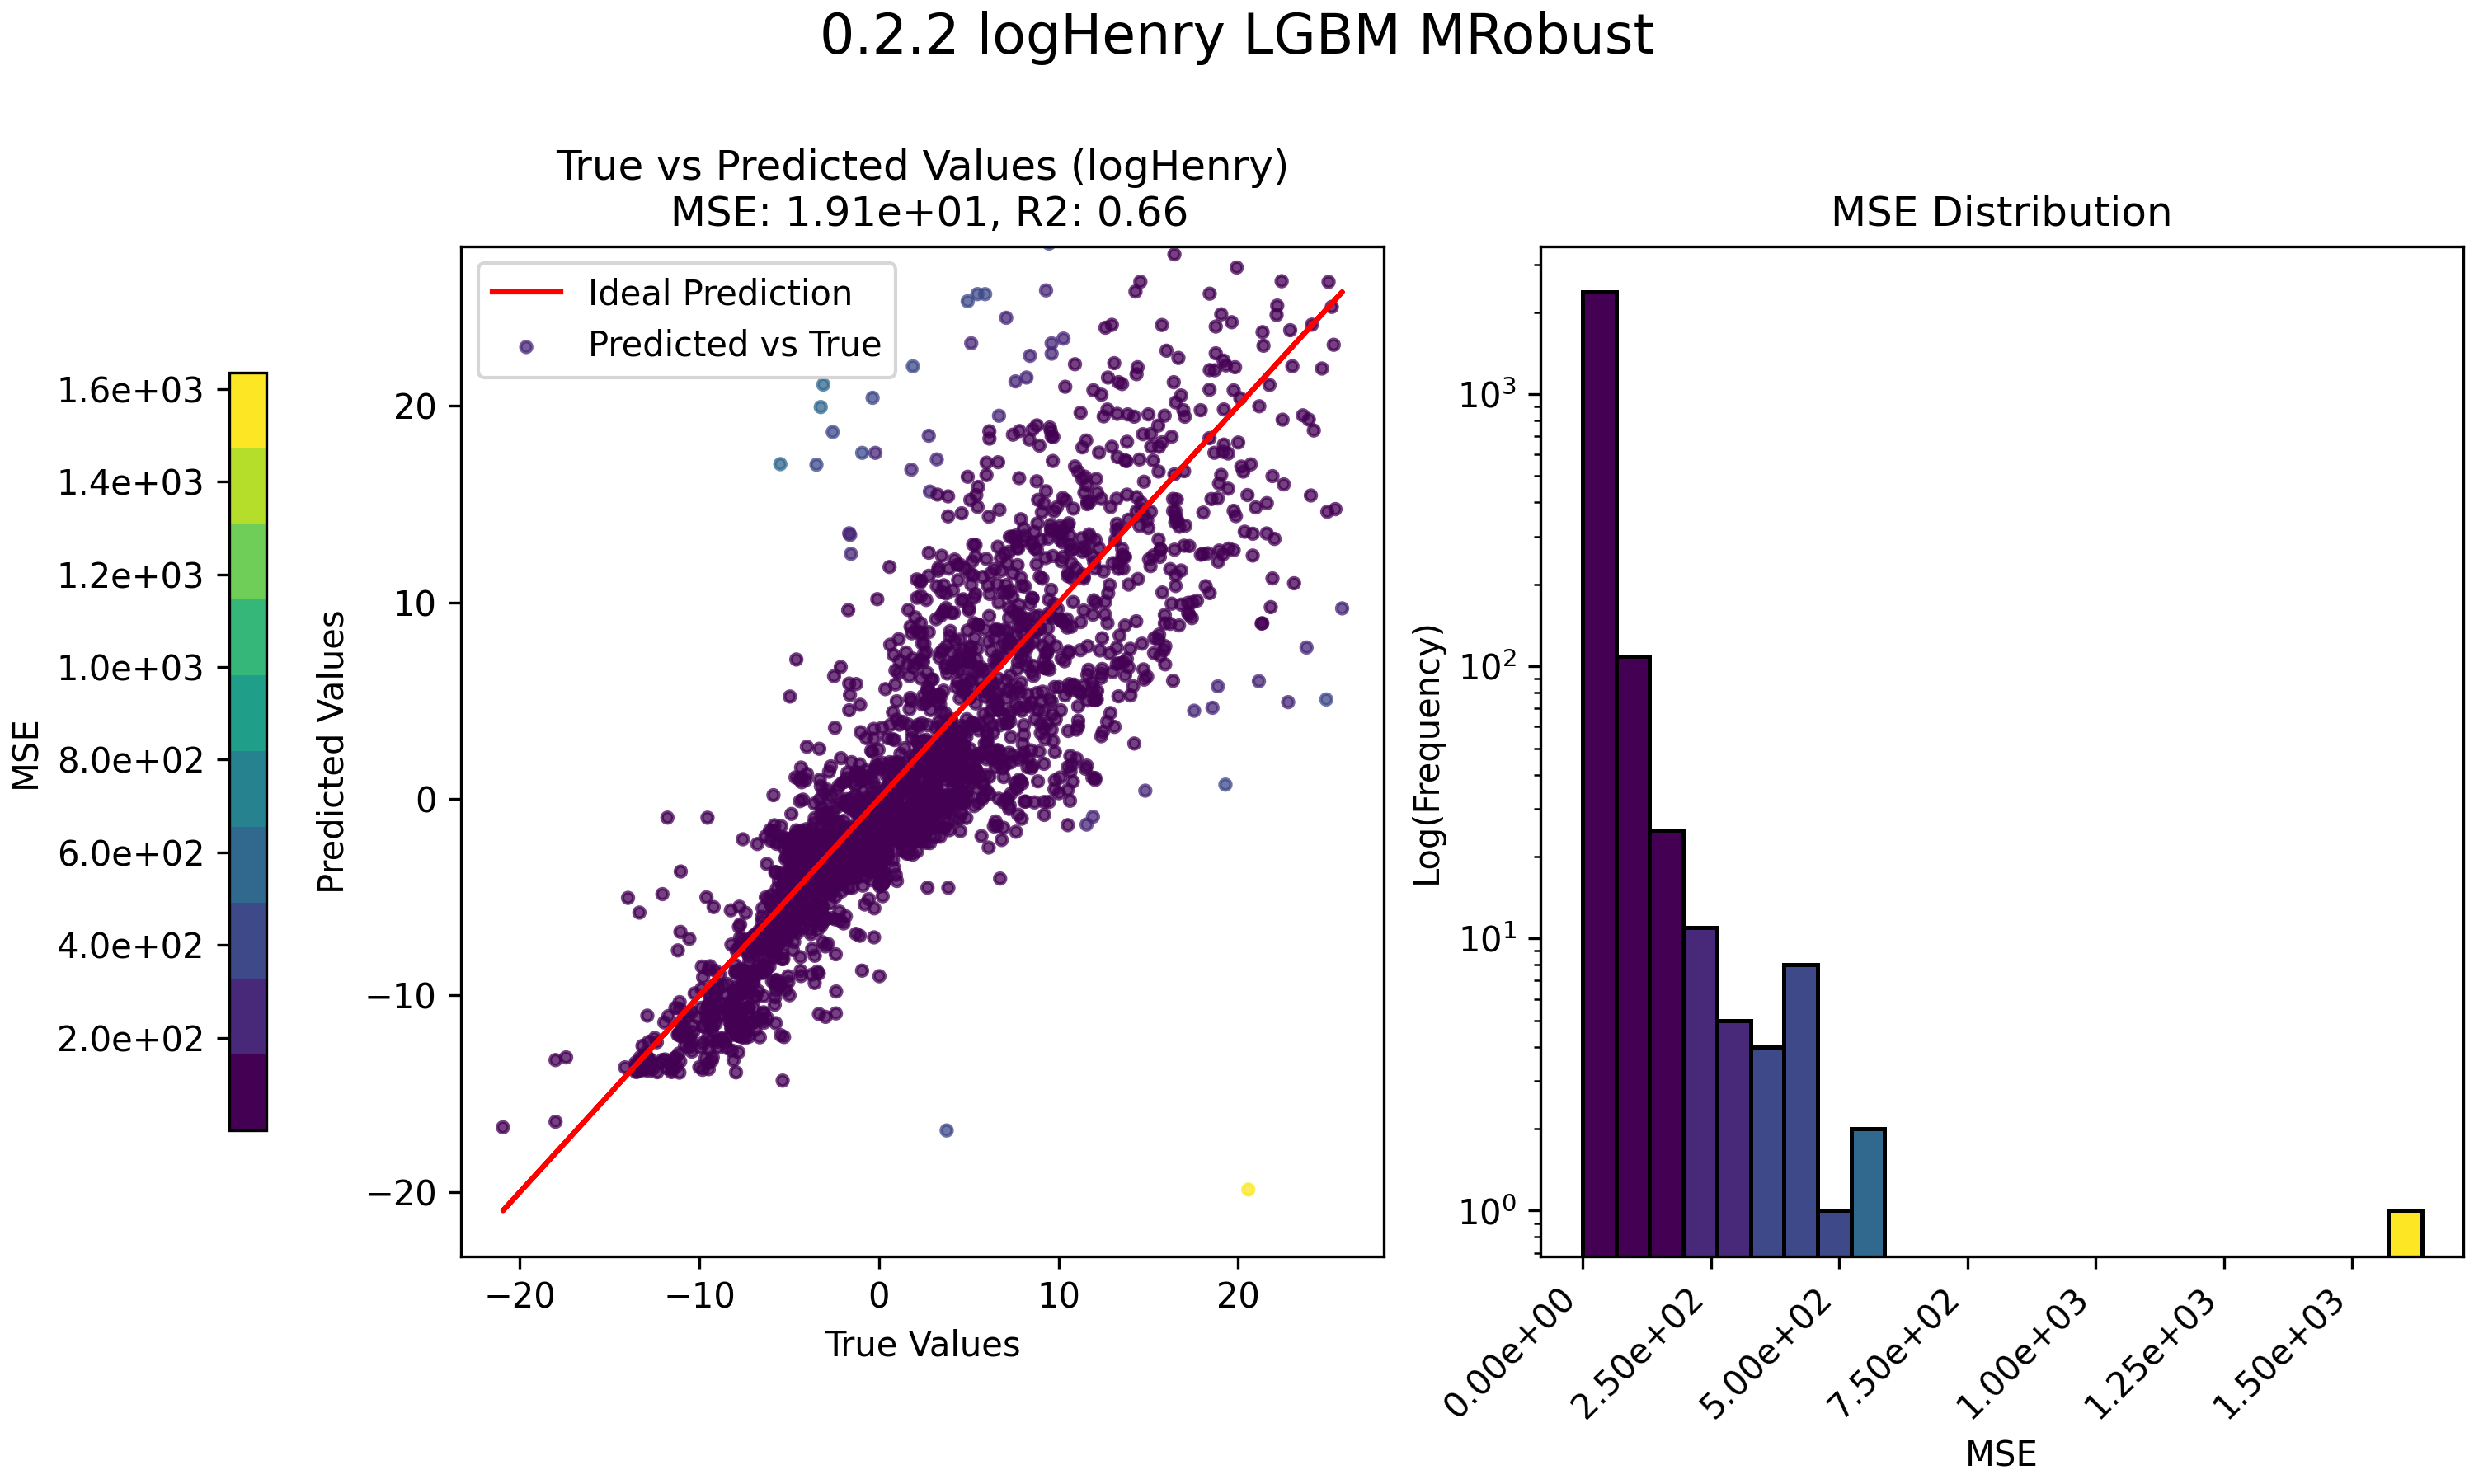
\includegraphics[width=0.8\linewidth]{figures/0.2.2-PredLogH.png}
	\caption{From left to right: the scatter plot of true versus predicted $\log k_H$ values for the test set (pred-set v0.2.2, dataset v0.7.1), and the distribution of the associated MSE for each prediction}
	\label{fig:PredLogH}
\end{figure}

\begin{figure}[H]
	\centering
	\small
	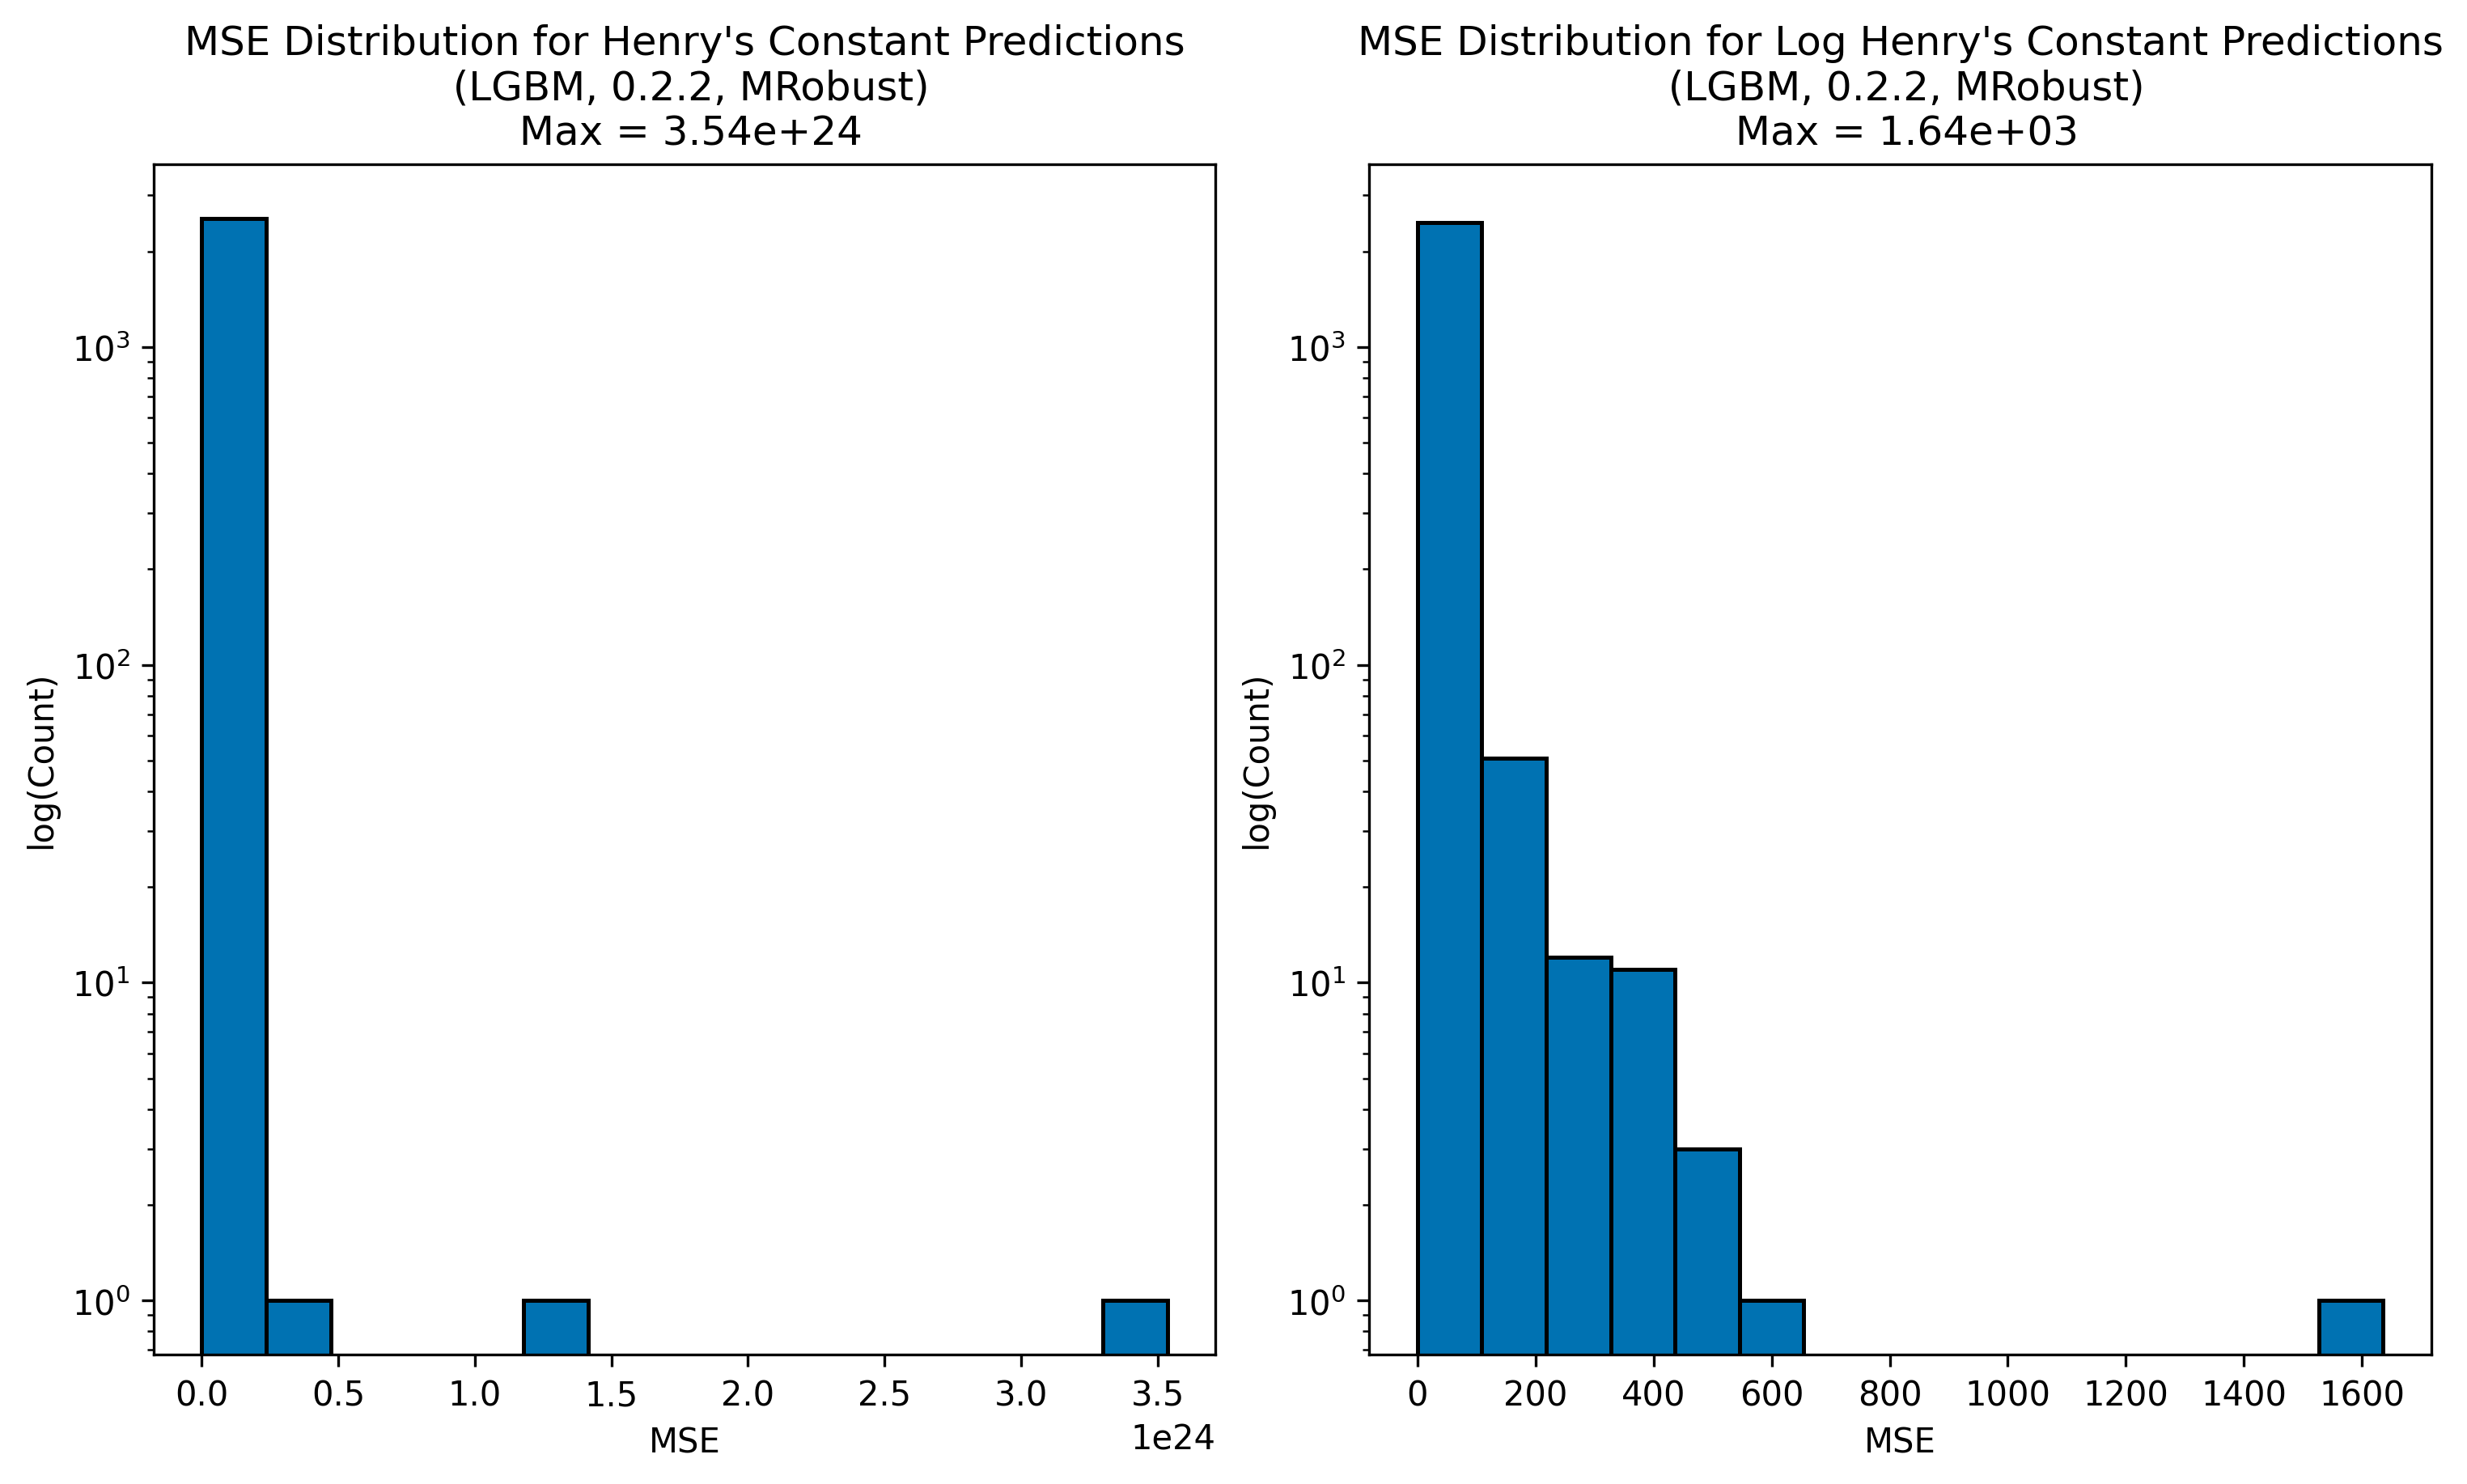
\includegraphics[width=0.8\linewidth]{figures/kH_MSE.png}
	\caption{The distribution of MSE values for each compound before and after the reverse log transform was applied to the predictions (pred-set v0.2.2, dataset v0.7.1)}
	\label{fig:kH_MSE}
\end{figure}

\begin{table}[H]
	\centering
	\small
	\begin{tabular}{|l|cc|}
		\hline
		\textbf{Metric} & \textbf{Log Transformed} & \textbf{Transform Reversed} \\
		\hline
		$\mathbf{R^2}$ & 0.66 & -68.67\\
		\textbf{MSE} & 19.11 & 2.13$\times10^{21}$ \\
		\textbf{\% MSE $>$ 1} & 76.53\% & 52.93\% \\
		\hline
	\end{tabular}
	\caption{A comparison of scores before and after reversing the log transform on the target variable ($k_H$), predset v0.2.2, dataset v0.7.1}
	\label{tab:kHScoreComparison}
\end{table}

The top and worst 10 predictions were compared for the transformed and reverse transformed target variable. There was no overlap between the 10 worst predicted compounds, but an overlap of 3 compounds for the best predicted compounds. 

\begin{figure}[H]
	\centering
	\begin{minipage}{0.3\textwidth}
		\centering\small
		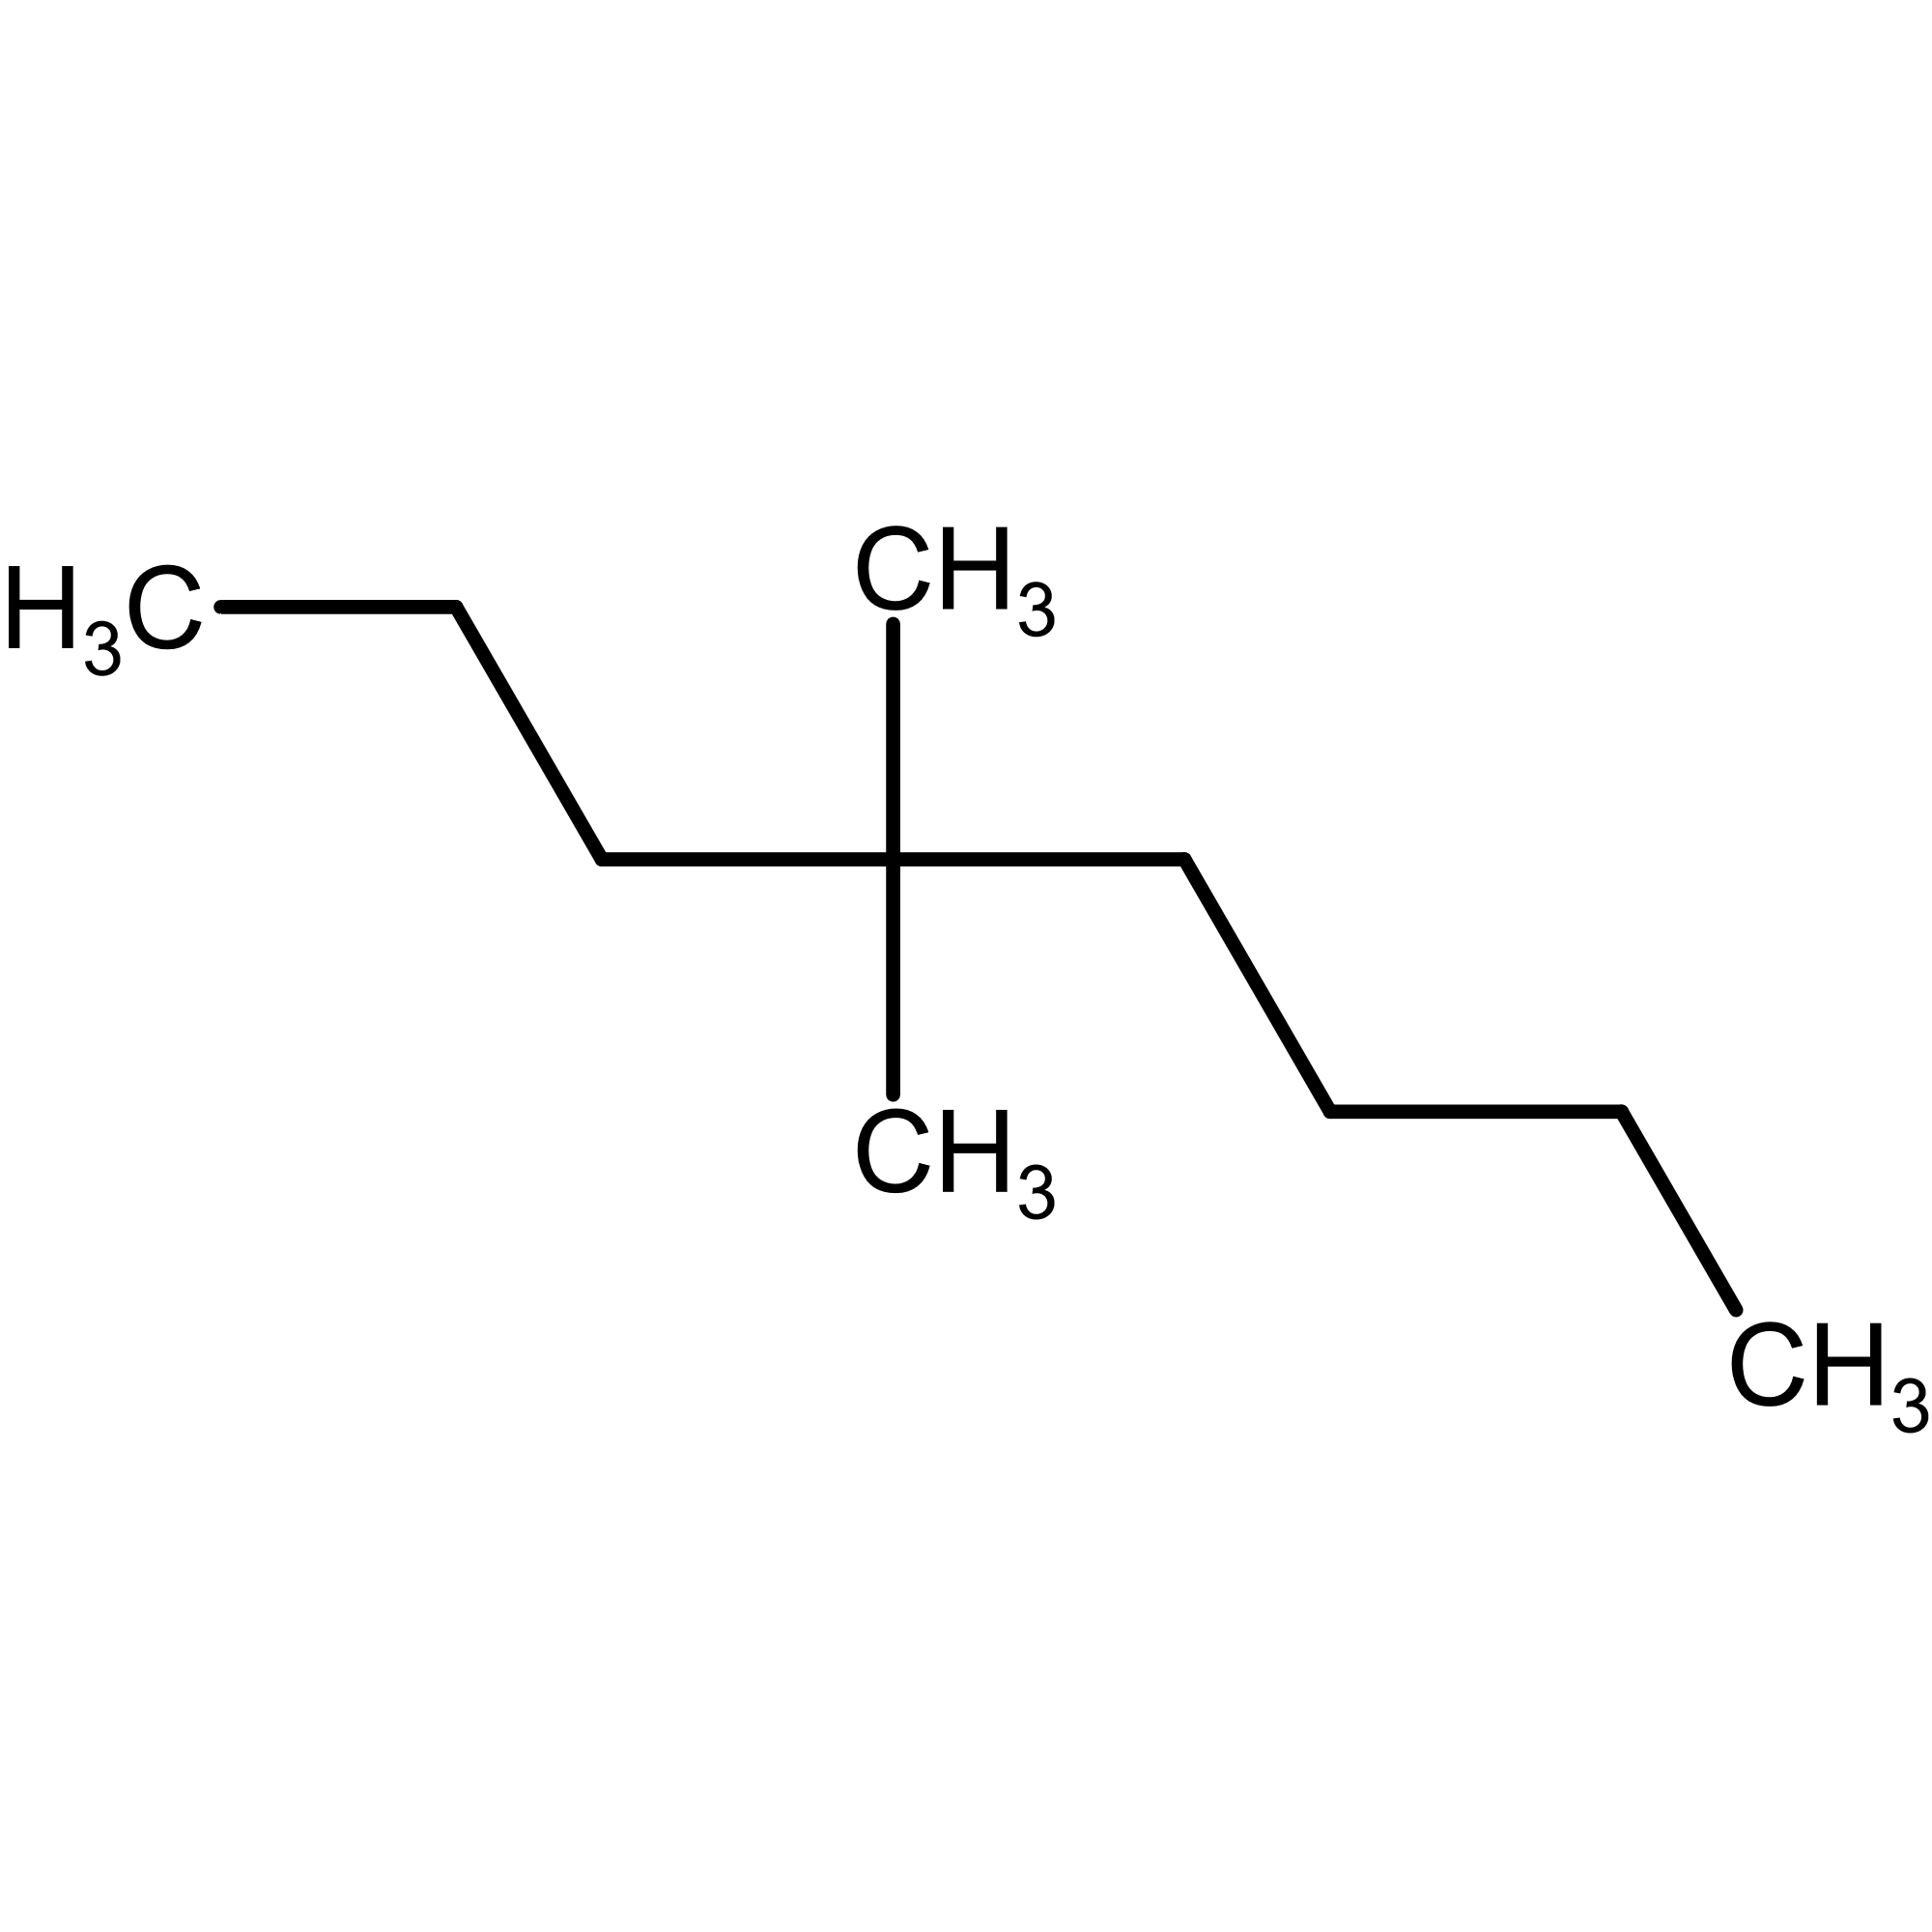
\includegraphics[width = 0.95\linewidth]{figures/HenryBest1.png}
	\end{minipage}
	\begin{minipage}{0.3\textwidth}
		\centering\small
		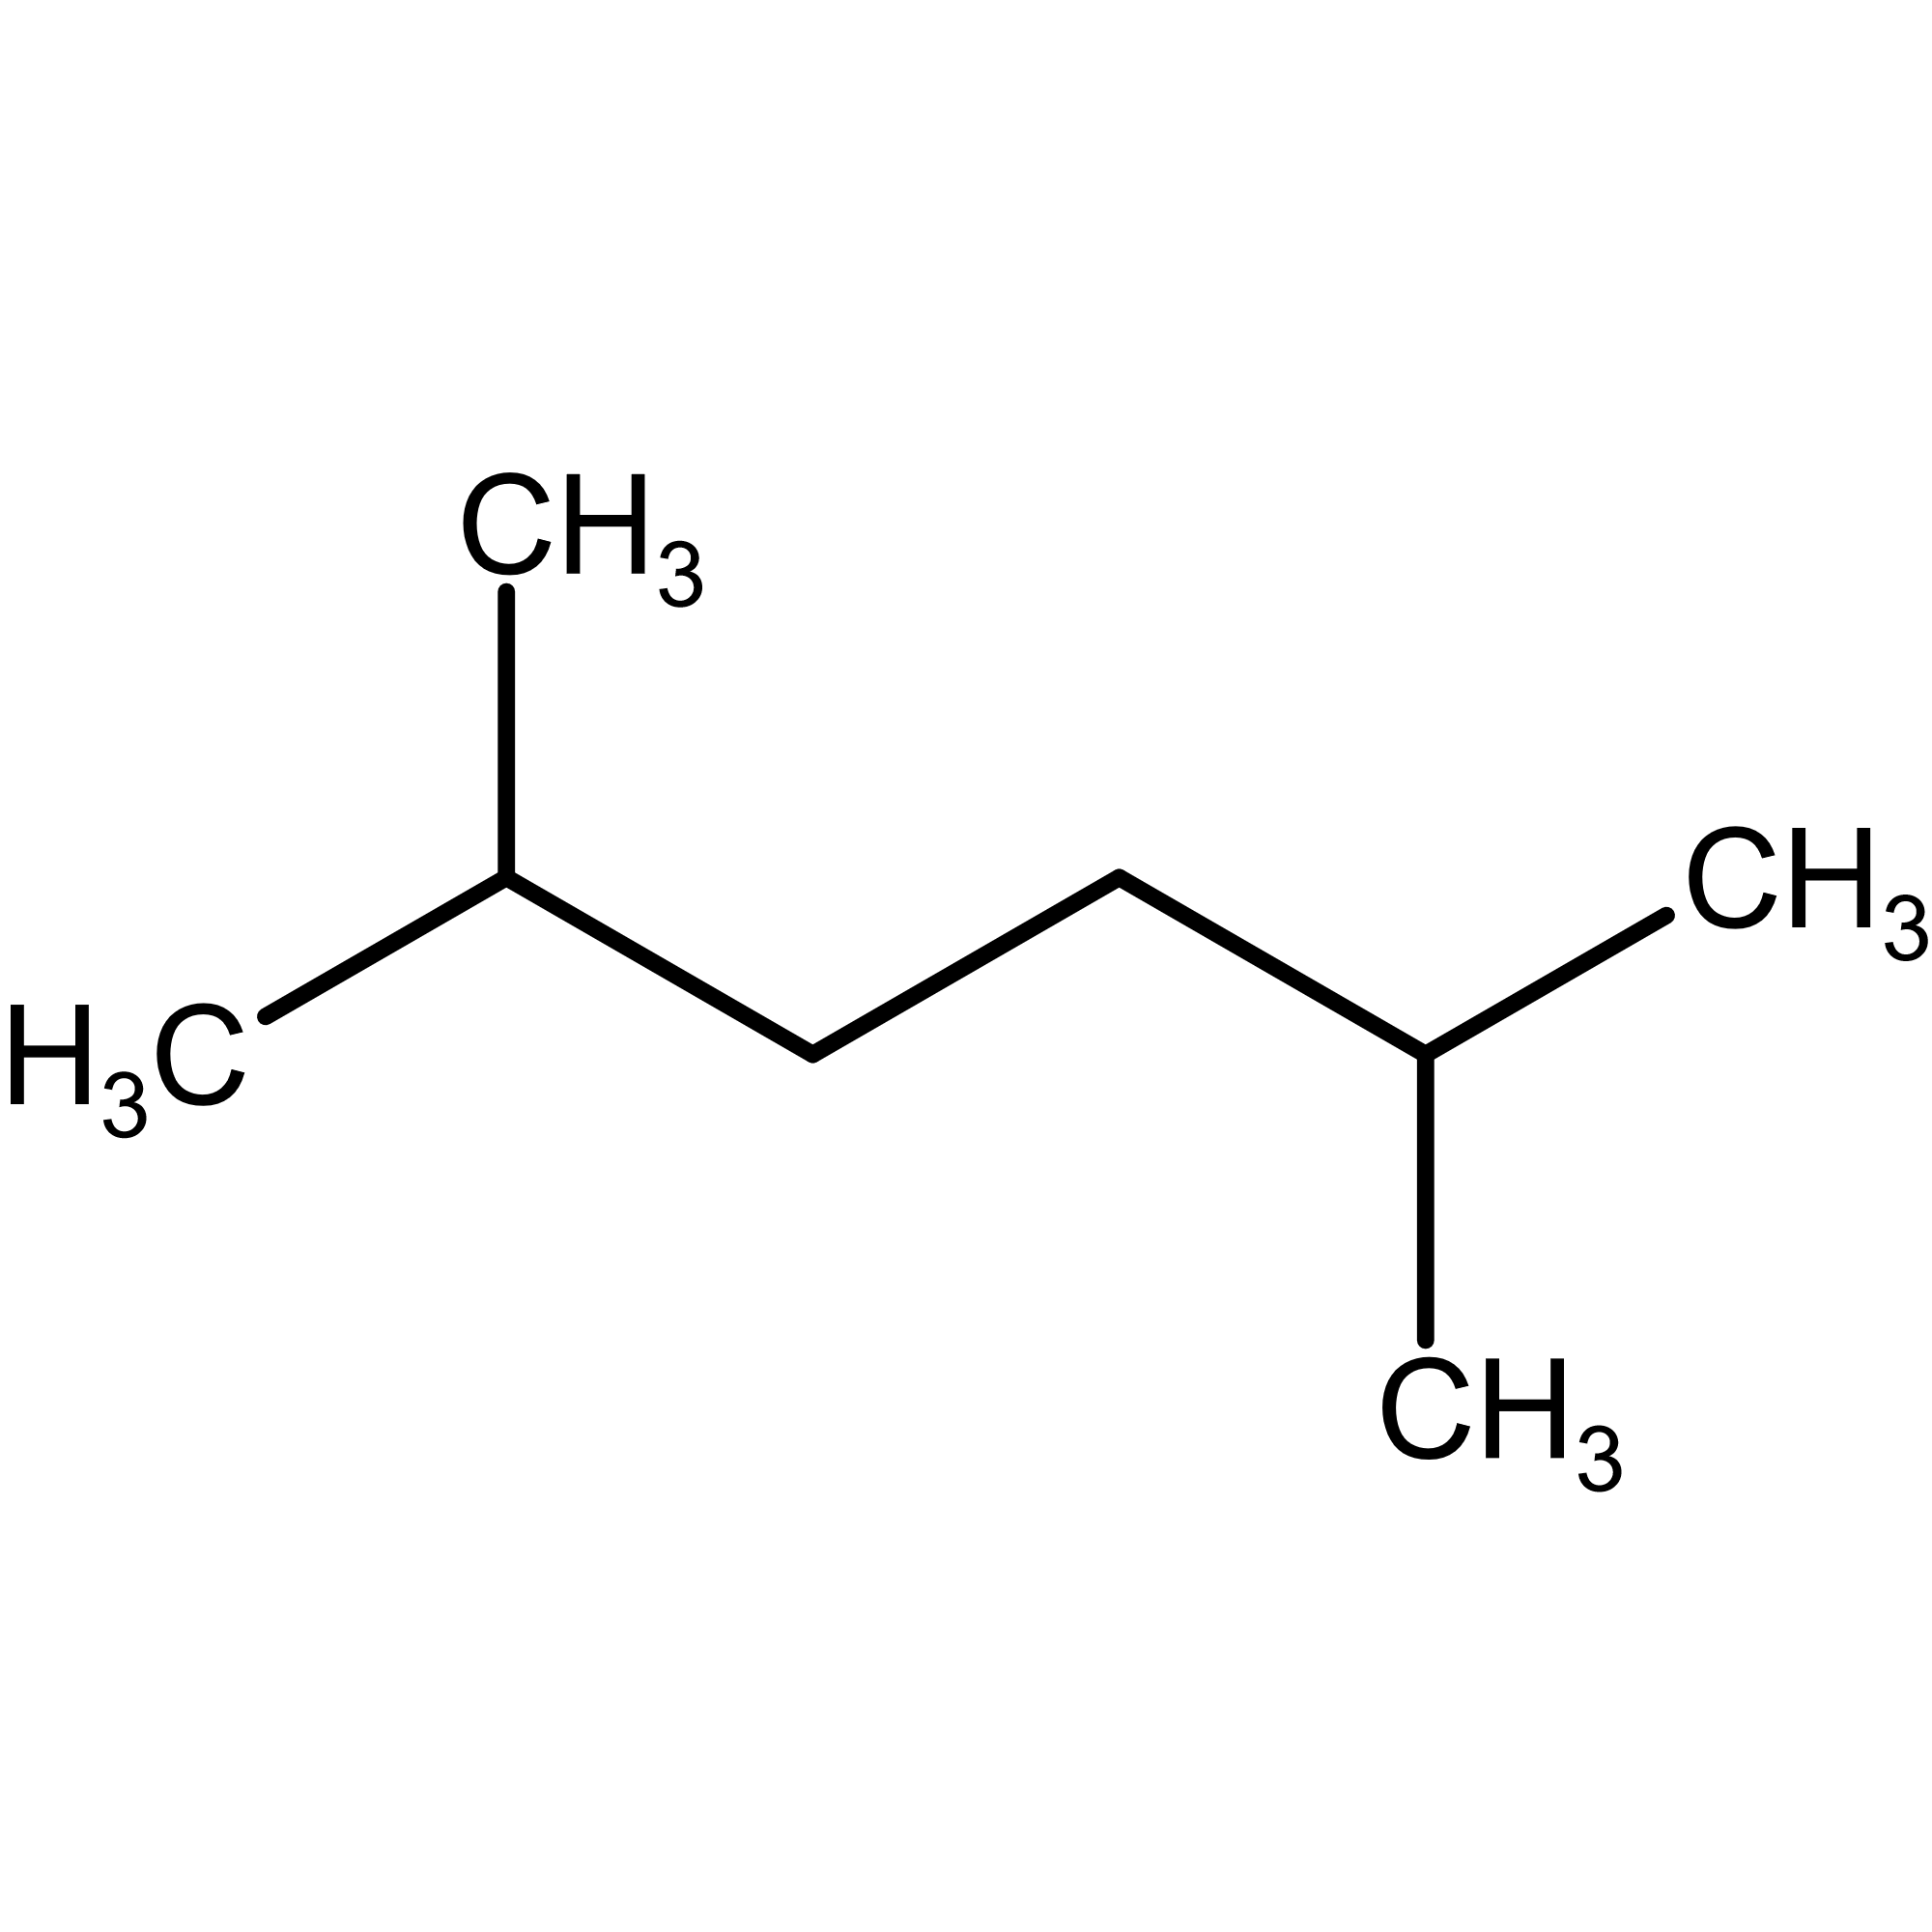
\includegraphics[width = 0.95\linewidth]{figures/HenryBest2.png}
	\end{minipage}
	\begin{minipage}{0.3\textwidth}
		\centering\small
		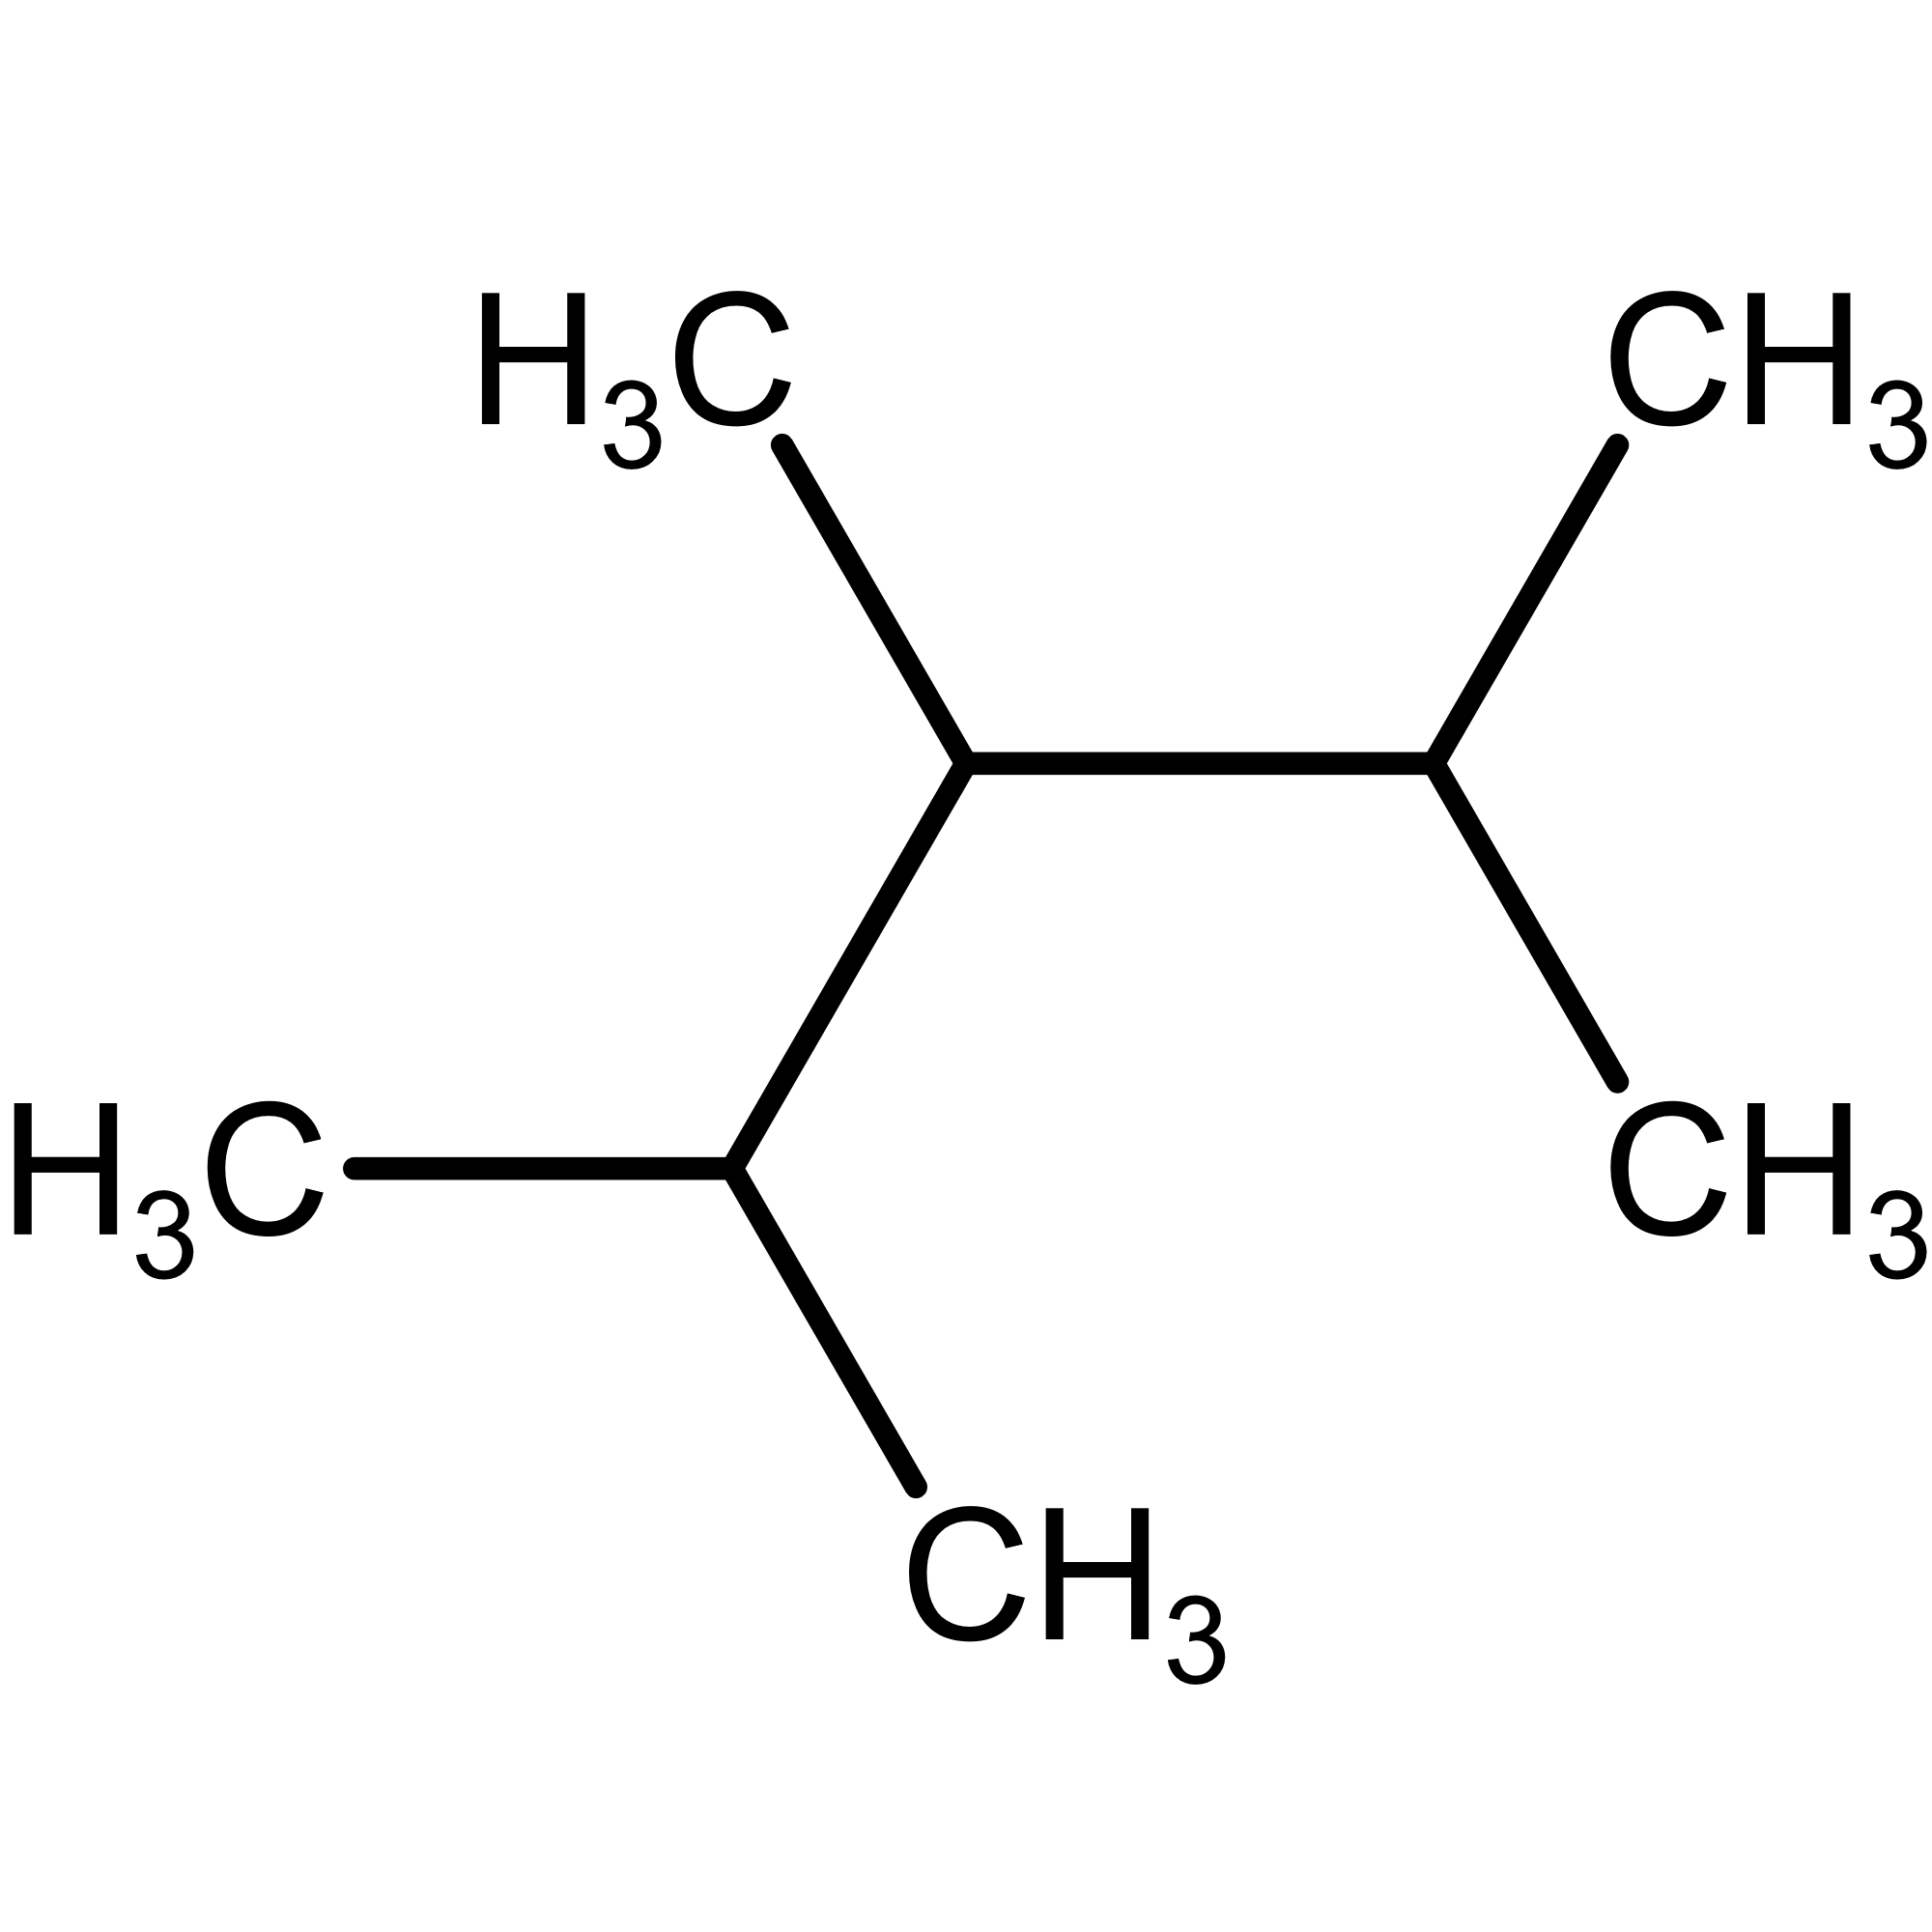
\includegraphics[width = 0.95\linewidth]{figures/HenryBest3.png}
	\end{minipage}
	\caption{The compounds that are in the top 10 most accurate predictions for log transformed and reverse transformed Henry's law constant}
\end{figure}

All of the compounds in the overlap are hydrocarbons and alkanes, meaning that they only contain hydrogen and oxygen. The alkane homologous series has a moderately fixed trend and chemical properties, so it is unsurprising that the overlapping compounds are all the same type. One of the reasons for this could be an overabundance of molecules with hydrocarbon fragments in the training set. This is analysed further in the following section (\ref{subsec:FuncGroupAnalysis}).

\subsection{Representation of Functional Groups in the Datasets}
\label{subsec:FuncGroupAnalysis}

\begin{figure}[H]
	\centering\small
	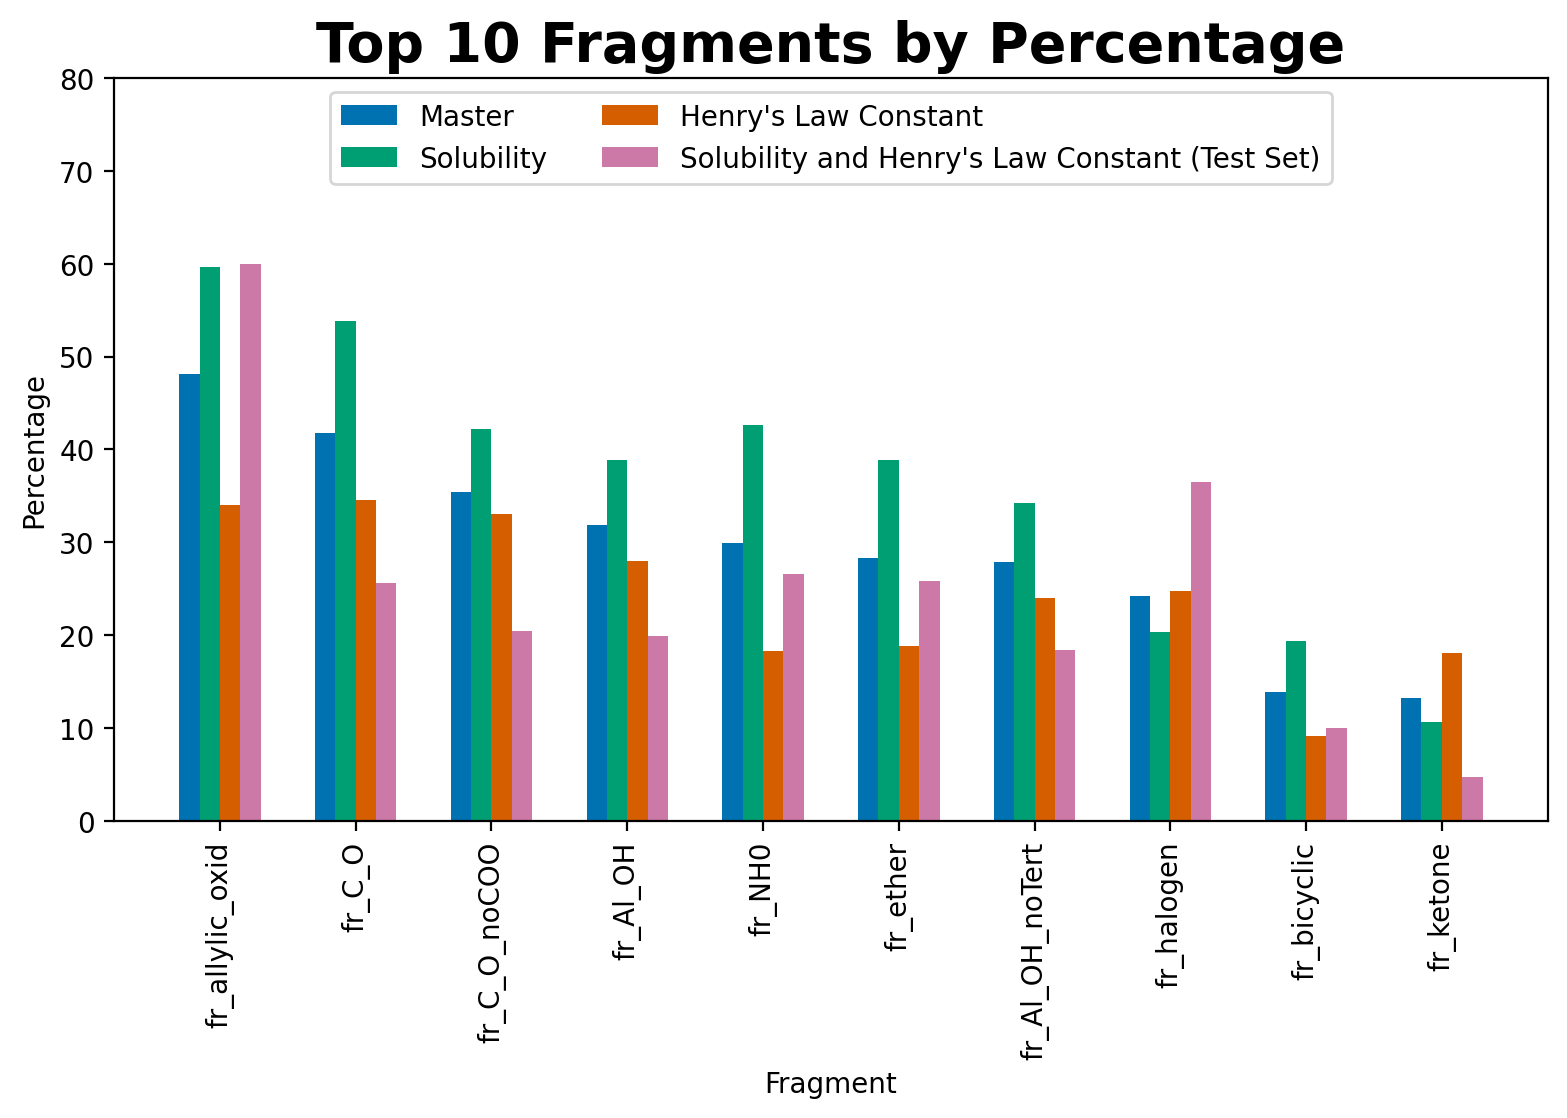
\includegraphics[width=0.9\linewidth]{figures/FuncGroupAnalysis.png}
	\caption{A comparison of the frequency percentage of the top 10 fragments in the master dataset, and the other datasets (v0.7.1)}
	\label{fig:FuncGroupAnalysis}
\end{figure}

Ideally, the percentage of compounds in a dataset with a specific fragment, e.g. \textit{fr\_C\_O}, should be the same as the test set. However, this is often not the case, with some fragments appearing nearly twice as often in the test set as the training set, like \textit{fr\_allylic\_oxid} in the Henry's law Dataset. This may have contributed to the poor scores when using the test set for certain subsets of compounds, as the test set was not randomly chosen. Further work is required to determine why particular compound and functional groups were predicted well, or poorly, by the models. Due to time constraints, this analysis has not been completed.

\section{Limitations and Challenges}
\label{sec:LimitationsChallenges}
There were many challenges throughout the course of the project, which were mostly data related. For Henry's law constant, there was only one dataset widely available. Out of 45 221 datapoints, 90\% (40 862) datapoints had no corresponding temperature. Those with no listed corresponding temperature were assumed to be at 25$^\circ$ C. Additionally, many had unknown CAS or InChI keys, which had to be resolved using various different python libraries. One library in particular, CIRpy, had a tendency to replace unresolved identifiers with water. Whilst this was simple to fix, as all datasets should not contain water, it was not identified until dataset version 0.6.0. The original scope of the project was too broad, and lead to time management issues. 

\section{Conclusion}
\label{sec:Conclusion}
Two models were developed simultaneously using the same processes to predict solubility and Henry's law constant. A dataset was compiled, containing both target variables, and a test set of the intersection of the datasets was set aside. The models were trained on the data that only contained the specific target variable (9 140 and 9 506 datapoints respectively), and tested on the shared data (2 563 datapoints). Both models achieved an acceptable level of accuracy and precision, with approximately 50\% of predictions in each test set scoring lower than 1 for MSE. For an unknown reason, the model to predict Henry's law constant performs exceptionally well for hydrocarbons, with MSE in the range of $10^{-5} - 10^{-6}$. Due to limited time available, the links between which features contribute best to predictions for each property were not investigated, and this aim was not fulfilled. This work will hopefully be completed in the future.

Flaws were identified in the way that the final models were developed, and there are definite opportunities for further enhancement of their performance. Furthermore, like in many machine learning projects, there were significant challenges with data, both in terms of quantity and quality. Data sanitation could be improved, however there is only so much data that can be gathered on the internet as a whole.

To further investigate what features contribute to the models' prediction ability, recursive feature elimination could be used to rank feature importance. This could be compared to the feature ranking by SelectKBest (with corrected scoring to use a regression based scorer rather than classification). To explore which compounds had the most accurate predictions, further analysis of fragments could be performed, and how it links with other features in the dataset. An uneven distribution of functional groups could be combated by methods such as oversampling, and data augmentation.

Further expansion could be completed by the inclusion of melting and boiling point data, testing how they work as features and targets for $\log S$ and $k_H$. Additionally, the links between phase diagrams and calculation of $k_H$ could be explored. Another possible route to explore would be to trial different representations of the molecules, rather than solely using the base RDKit 2D descriptors.

%%Outputs, Data & Software Links here
\section{Outputs, Data \& Software Links}
\label{sec:outputs}
%\textit{Guidance (Delete upon completion): If you have produced any outputs (including poster presentations, GitHub repositories of data or software produced etc) please include details and links to these. These links must be accessible. If you have specific reasons why your data / outputs are not able to be made more available then this should be discussed with your supervisor and details provided in the report.}

All the data, scripts, results, and other outputs are available at \url{https://github.com/joooshc/PSDI_HLC}. Anything containing solubility data has been removed due to copyright issues with DDB.

%% references here. If you have a .bib file or similar please also attach this to the email including the report.

% Add references for python, matplotlib, etc, using \nocite{key}
\nocite{python, matplotlib, numpy, scikit}
\bibliographystyle{vancouver}
\bibliography{References}

\section{Appendix}
\label{sec:Appendix}
\subsection{Feature Selection with SelectKBest}

\begin{table}[H]
	\centering\small
	\begin{tabular}{|c|c|c|}
		\hline
		\textbf{Num Features (k)} & $\mathbf{R^2}$ & \textbf{MSE}\\
		\hline
		1 & 0.00 & 54.5 \\
		98 & 0.86 & 7.48 \\
		146 & 0.87 & 6.93 \\
		170 & 0.87 & 6.93 \\
		182 & 0.88 & 6.39 \\
		\textbf{188} & \textbf{0.88} & \textbf{6.39} \\
		195 & 0.88 & 6.41 \\ 
		\hline
	\end{tabular}
	\caption{A table comparing the results for SelectKBest on the $\log k_H$ (v0.4.2) dataset. The highest scoring result is highlighted in bold.}
	\label{tab:SelectKBest}
\end{table}

\subsection{Principal Component Analysis (PCA)}
\label{subsec:PCA_Results}
\begin{table}
	\centering\small
	\begin{tabular}{|c|c|c|}
		\hline
		\textbf{Num Components} & $\mathbf{R^2}$ & \textbf{MSE} \\
		\hline
		1 & -0.74 & 78.76 \\
		61 & 0.15 & 38.40 \\
		91 & 0.18 & 37.06 \\
		106 & 0.19 & 36.83 \\
		114 & 0.20 & 36.39 \\
		122 & 0.20 & 36.38 \\
		\hline
	\end{tabular}
	\caption{The effect of PCA on model performance, dataset version 0.5.3.}
	\label{tab:PCA_Results}
\end{table}

\subsection{Scaling Results}

\begin{table}[H]
    \centering
    \begin{tabular}{|l|l|c|c|}
		\hline
        \textbf{Normalisation} & \textbf{Scaling} & \textbf{MSE} & $\mathbf{R^2}$ \\ 
		\hline
        None & None & 0.77 & 0.86 \\ 
        \textbf{MinMax} & \textbf{RobustScaler()} & \textbf{0.88} & \textbf{0.84} \\ 
        MinMax & normalize & 0.90 & 0.83 \\ 
        Normalize & normalize & 0.90 & 0.83 \\ 
        Normalize & PowerTransformer(standardize=False) & 0.95 & 0.82 \\ 
        MinMax & StandardScaler() & 0.96 & 0.82 \\ 
        Normalize & MaxAbsScaler() & 1.06 & 0.80 \\ 
        Normalize & RobustScaler() & 1.44 & 0.73 \\ 
        Normalize & StandardScaler() & 2.36 & 0.56 \\ 
        MinMax & MaxAbsScaler() & 4.86 & 0.09 \\ 
        MinMax & MinMax & 4.97 & 0.07 \\ 
        Normalize & MinMax & 4.97 & 0.07 \\ 
        MinMax & PowerTransformer(standardize=False) & 9.88 & -0.85 \\ 
		\hline
    \end{tabular}
	\caption{A comparison of the scaling methods trialled on the {$\log S$} dataset (v0.4.2) sorted by $R^2$, testing using the base LightGBM regressor. The scaling method chosen for the rest of the modelling is highlighted in bold.}
	\label{tab:ScalingLogS}
\end{table}

\begin{table}[H]
    \centering
    \begin{tabular}{|l|l|c|c|}
    \hline
        \textbf{Normalisation} & \textbf{Scaling} & \textbf{MSE} & $\mathbf{R^2}$ \\ 
		\hline
        None & None & 5.64 & 0.90 \\ 
        \textbf{MinMax} & \textbf{RobustScaler()} & \textbf{6.41} & \textbf{0.88} \\ 
		MinMax & StandardScaler() & 6.83 & 0.87 \\ 
        Normalize & normalize & 7.37 & 0.86 \\ 
        MinMax & normalize & 7.37 & 0.86 \\ 
        Normalize & MaxAbsScaler() & 7.64 & 0.86 \\ 
        Normalize & PowerTransformer(standardize=False) & 8.30 & 0.85 \\ 
        Normalize & RobustScaler() & 16.27 & 0.70 \\ 
        Normalize & MinMax & 40.63 & 0.25 \\ 
        MinMax & MaxAbsScaler() & 40.63 & 0.25 \\ 
        MinMax & MinMax & 40.63 & 0.25 \\ 
        MinMax & PowerTransformer(standardize=False) & 60.59 & -0.11 \\ 
        Normalize & StandardScaler() & 67.25 & -0.24 \\
		\hline
    \end{tabular}
	\caption{A comparison of the scaling methods trialled on the {$k_H$} dataset (v0.3.2) sorted by $R^2$, testing using the base LightGBM regressor. The scaling method chosen for the rest of the modelling is highlighted in bold.}
	\label{tab:ScalingLogH}
\end{table}

\subsection{Model Hyper-parameters}
\label{subsec:ModelHyperparameters}

\begin{table}[H]
	\centering\small
	\begin{tabular}{|l|c|c|}
		\hline
		\textbf{Parameter} & $\log S$ & $\mathbf{\log k_H}$ \\
		\hline
		n\_estimators & 200 & 100 \\
		learning\_rate & 0.1 & 0.2 \\
		loss & exponential & exponential\\
		\hline
	\end{tabular}
	\caption{The hyper-parameters used for AdaBoost Regressor}
	\label{tab:AdaBoost_params}
\end{table}

\begin{table}[H]
	\begin{minipage}{.5\linewidth}
		\centering\small
		\begin{tabular}{|l|c|c|}
			\hline
			\textbf{Parameter} & $\log S$ & $\mathbf{k_H}$ \\
			\hline
			boosting\_type & gbdt & gbdt \\
			n\_estimators & 600 & 600 \\
			num\_leaves & 31 & 31 \\
			max\_bin & 255 & 244 \\
			num\_threads & 4 & 4 \\
			learning\_rate & 0.1 & 0.05 \\
			\hline
		\end{tabular}
		\caption{The hyper-parameters used for LightGBM Regressor}
		\label{tab:LGBM_params}
	\end{minipage}
	\begin{minipage}{.5\linewidth}
		\centering\small
		\begin{tabular}{|l|c|c|}
			\hline
			\textbf{Parameter} & $\log S$ & $\mathbf{k_H}$ \\
			\hline
			boosting\_type & rf & rf \\
			n\_estimators & 400 & 600 \\
			num\_leaves & 50 & 31 \\
			max\_bin & 255 & 255 \\
			num\_threads & 4 & 4 \\
			learning\_rate & 0.1 & 0.05 \\
			bagging\_freq & 4 & 1 \\
			bagging\_fraction & 0.8 & 0.8 \\
			\hline
		\end{tabular}
		\caption{The hyper-parameters used for Random Forest}
		\label{tab:rf_params}
	\end{minipage}
\end{table}

\begin{table}[H]
	\begin{minipage}{.5\linewidth}
		\centering\small
		\begin{tabular}{|l|c|c|}
			\hline
			\textbf{Parameter} & $\log S$ & $\mathbf{k_H}$ \\
			\hline
			kernel & laplacian & laplacian\\
			alpha & 0.05 & 0.04\\
			\hline
		\end{tabular}
		\caption{The hyper-parameters used for Kernel Ridge Regression}
		\label{tab:KRR_params}
	\end{minipage}
	\begin{minipage}{.5\linewidth}
		\centering\small
		\begin{tabular}{|l|c|c|}
			\hline
			\textbf{Parameter} & $\log S$ & $\mathbf{k_H}$ \\
			\hline
			n\_neighbors & 9 & 5 \\
			weights & distance & distance \\
			p & 1 & 1\\
			\hline
		\end{tabular}
	\end{minipage}
\end{table}

\begin{table}[H]
	\centering\small
		\begin{tabular}{|l|c|c|}
			\hline
			\textbf{Parameter} & $\log S$ & $\mathbf{k_H}$ \\
			\hline
			kernel & linear & linear \\
			C & 1.0 & 1.0\\
			epsilon & 0.1 & 0.4 \\
			\hline
		\end{tabular}
		\caption{The hyper-parameters used for model X}
		\label{tab:SVR_params}
\end{table}


\end{document}